\documentclass[journal]{IEEEtran}

% ============================================================
% MFFT — JOURNAL MANUSCRIPT (PILOT/SMOKE-TEST RESULTS)
% ------------------------------------------------------------
% Every number in this manuscript is traceable to project artifacts:
%   paper/result/test/{tiny,base,large}_model/table/*.json   (primary pilot run)
%   paper/result/test/ablation/ablation_summary.csv          (component ablation)
%   paper/result/test/baselines_model/baseline_summary.csv   (10 baselines)
%   paper/result/verify/logo/logo_summary.csv                (LOGO probes)
%   paper/result/verify/paper_evals/*.csv                    (robustness, CI,
%                                                              McNemar, calibration)
%   paper/result/verify/ablation/upgrade_*.json              (extension ablation)
% Pilot protocol: 1 epoch, 5,000-image subset (4,000/500/500), 224x224.
% ============================================================

\usepackage{amsmath}
\usepackage{amssymb}
\usepackage{cite}
\usepackage{graphicx}
\usepackage{url}
\usepackage{array}
\usepackage{booktabs}
\usepackage{multirow}
\usepackage{xcolor}
\usepackage{algorithm}
\usepackage{algorithmic}
\usepackage{tikz}
\usetikzlibrary{positioning,arrows.meta,calc,fit,backgrounds}

\hyphenation{op-tical net-works semi-conduc-tor fre-quen-cy de-com-po-si-tion ge-ne-ra-tive ad-ver-sar-i-al}

\begin{document}

\title{Multi-Frequency Fusion Transformer for AI-Generated Image Detection: Architecture, Controlled Pilot Evaluation, and Cross-Generator Analysis}

\author{Mohsin~Ibna~Hossain,~MD.~Muttakin,~and~Mohammad~Mahmudul~Hasan,~\IEEEmembership{Member,~IEEE}%
\thanks{M. I. Hossain and MD. Muttakin are with the Department of Computer Science, American International University-Bangladesh, Dhaka, Bangladesh (e-mail: 23-50194-1@student.aiub.edu; 23-50987-1@student.aiub.edu).}%
\thanks{M. M. Hasan is with the Department of Computer Science, American International University-Bangladesh, Dhaka, Bangladesh (e-mail: m.hasan@aiub.edu).}}

\markboth{Journal Manuscript, 2026}%
{Hossain \MakeLowercase{\textit{et al.}}: Multi-Frequency Fusion Transformer for AI-Generated Image Detection}

\maketitle

\begin{abstract}
The arrival of rectified-flow generators and natively multimodal language models has pushed synthetic imagery past the threshold of reliable human discrimination, while recent benchmark audits show that many published detectors collapse on images from unseen generators and real-world distributions. Existing detectors predominantly operate in the spatial domain, yet generative pipelines leave characteristic traces in the frequency domain that are complementary to spatial cues and rooted in the mathematics of the generation process itself. We present the Multi-Frequency Fusion Transformer (MFFT), an architecture that decomposes an input image into low, mid, and high frequency bands via differentiable Fourier-based radial filtering, extracts per-band features with dedicated lightweight CNN backbones using depthwise separable convolutions, and fuses the bands through multi-head cross-attention augmented by a Frequency-Guided Attention (FGA) gating mechanism grounded in the physical spectral energy of the input. Three variants---MFFT-Tiny (372K), MFFT-Base (1.62M), and MFFT-Large (6.30M parameters)---span an accuracy--efficiency trade-off with 1.5--25~MB checkpoints suitable for edge-to-server deployment. We report a controlled \emph{pilot study}: all models are trained for a single epoch on a balanced 5,000-image subset of our 2.7-million-image corpus and evaluated against ten baselines under an identical protocol. Trained from scratch, MFFT-Large reaches 91.4\% accuracy (0.964 AUC), outperforming every other from-scratch model by a wide margin (best competitor: 77.2\%) while remaining within 4--7 points of ImageNet-pretrained CNNs that use 2--14$\times$ more parameters. Ablations over thirteen configurations show that frequency decomposition is the dominant factor: every multi-band fusion strategy outperforms a spatial-only control by 5--9 points at identical parameter count. We further demonstrate the complete evaluation protocol a full-scale study requires---leave-one-generator-out probes across eight generator families (mean balanced accuracy 78.9\%), a post-processing robustness suite showing strong JPEG stability but vulnerability to downscaling and blur, temperature-scaled calibration (ECE $0.059 \rightarrow 0.029$), bootstrap confidence intervals, and McNemar significance testing. The architecture additionally yields intrinsic, independently reproducible per-band anomaly heatmaps for interpretable forensic evidence. Code, data manifests, and checkpoints will be released.
\end{abstract}

\begin{IEEEkeywords}
AI-generated image detection, image forensics, frequency analysis, cross-attention fusion, deepfake detection, vision transformer, generalization, interpretability, model calibration.
\end{IEEEkeywords}

\IEEEpeerreviewmaketitle

% ============================================================
\section{Introduction}
% ============================================================
\IEEEPARstart{M}{odern} generative models---latent diffusion systems such as Stable Diffusion~\cite{rombach2022}, rectified-flow transformers such as Stable Diffusion~3 and FLUX~\cite{esser2024}, adversarial models in the StyleGAN family~\cite{karras2019}, and natively multimodal language models with built-in image generation---now produce images that human observers cannot reliably distinguish from photographs. This capability threatens journalism, legal evidence, biometric security, scientific integrity, and public discourse. Synthetic imagery has been documented in election disinformation, fabricated news, identity fraud, and large-scale social engineering, and the volume of AI-generated content circulating on public platforms continues to grow~\cite{croitoru2024,pei2026survey}. Human inspection does not scale and is unreliable: studies consistently find that untrained observers perform near chance on high-quality diffusion outputs. Automated detection is therefore a foundational requirement for media-authenticity infrastructure~\cite{wang2020,ojha2023,zhu2023genimage,tan2024npr}.

A central and still unsolved difficulty is \emph{generalization}. Detectors trained on one family of generators degrade sharply on unseen families~\cite{ojha2023,corvi2023,yan2025sanity}: accuracy drops of 15--25 points are routinely reported when a GAN-trained detector meets diffusion outputs. Two recent audits sharpen the point. The Chameleon in-the-wild evaluation~\cite{yan2025sanity} found most published detectors near chance on images collected outside their benchmark distribution, and the AIGIBench audit~\cite{li2025aigibench} reached the same conclusion across 23 generator subsets and social-media re-shares: high leaderboard accuracy does not survive contact with deployment conditions. A growing body of 2025--2026 work attributes much of this failure to \emph{semantic shortcuts}---detectors latching onto content categories or stylistic regularities of the training generators rather than forensic traces~\cite{shuai2026shortcuts}. Spatial-domain classifiers are especially exposed: when the generator or content distribution changes, the learned shortcut disappears.

Frequency-domain analysis offers a more principled signal. Upsampling operations common to CNN-based decoders imprint periodic artifacts in the high-frequency spectrum~\cite{zhang2019wifs,durall2020,frank2020}; diffusion models systematically distort mid-to-high frequency statistics relative to natural images~\cite{corvi2023,ricker2024}; and all synthetic pipelines lack the sensor-noise signature that a physical camera imprints on real photographs~\cite{cozzolino2019}. Because these traces originate in the mathematics of the generation process---transposed convolutions, decoder upsampling factors, denoising trajectories---rather than in the training data of any particular model, they are plausible candidates for architecture-agnostic detection cues. Frequency-aware detectors such as FreqNet~\cite{tan2024freqnet}, NPR~\cite{tan2024npr}, and the dual-frequency-branch framework of Yan \textit{et al.}~\cite{yan2026dualfreq} exploit exactly this intuition and report among the strongest cross-generator results in the current literature.

\subsection{Motivation: Why \emph{Multiple} Bands}
Existing frequency-based methods typically operate on a single high-pass residual, a full-spectrum representation, or aggregate spectral statistics, discarding the multi-scale structure of the spectrum. Yet the forensic literature indicates that different generator families concentrate their artifacts in \emph{different} frequency ranges. GAN upsampling artifacts---checkerboard patterns from transposed convolutions---are predominantly high-frequency~\cite{zhang2019wifs,durall2020}. Diffusion denoising signatures span mid-to-high bands, reflecting the mismatch between the training-time noise schedule and the inference-time sampling trajectory~\cite{corvi2023}. Structural anomalies of autoregressive and patch-based generators manifest at low frequencies as global-coherence failures. A single-band detector is blind to whichever artifacts fall outside its band; an aggregate-spectrum detector dilutes localized band evidence into global statistics. A detector that \emph{adaptively weights multiple frequency bands per input} should therefore be more robust than any single-band scheme---this is the hypothesis MFFT is designed to test.

A second motivation is efficiency. State-of-the-art universal detectors increasingly rely on frozen foundation-model backbones (CLIP ViT-L, DINOv2) with hundreds of millions of parameters~\cite{ojha2023,tan2025c2pclip,yan2025effort}. Platform-scale screening---millions of images per day---and on-device deployment require far smaller models. If explicit frequency decomposition supplies the inductive bias that large backbones otherwise learn from data, compact frequency-native architectures may achieve competitive accuracy at a fraction of the cost.

\subsection{Contributions}
We propose the Multi-Frequency Fusion Transformer (MFFT) and make the following contributions:
\begin{enumerate}
    \item \textbf{Multi-band frequency decomposition:} a differentiable, non-parametric FFT-based module that splits the input into low, mid, and high radial frequency bands, each processed by a dedicated lightweight CNN with depthwise separable convolutions (Algorithm~\ref{alg:forward}).
    \item \textbf{Cross-attention band fusion (CAF):} a multi-head attention mechanism over band tokens that learns input-dependent inter-band relationships, replacing static fusion rules such as concatenation or pooling.
    \item \textbf{Frequency-Guided Attention (FGA):} a gating mechanism that weights fused features by the physical frequency-magnitude content of the input, providing an inductive bias grounded in spectral energy rather than learned correlations alone---a design that directly targets the semantic-shortcut failure mode~\cite{shuai2026shortcuts}.
    \item \textbf{Three efficient variants} spanning 372K--6.30M parameters with 1.5--25~MB checkpoints, plus three architecture extensions (ImageNet-pretrained band extractors, an NPR-style high-band residual~\cite{tan2024npr}, and soft band masks) evaluated in ablation.
    \item \textbf{Pilot-scale controlled evaluation:} a single-protocol comparison against ten baselines---from-scratch CNNs and ViTs, ImageNet-pretrained CNNs and transformers, CLIP linear probing, and a hand-crafted spectral method---together with a thirteen-configuration ablation isolating each architectural component.
    \item \textbf{A complete generalization and rigor protocol}, demonstrated end to end at pilot scale: leave-one-generator-out (LOGO) evaluation across eight generator families (Algorithm~\ref{alg:logo}), a JPEG/downscale/blur robustness suite, temperature-scaled calibration, bootstrap confidence intervals, and McNemar significance testing.
    \item \textbf{Intrinsic interpretability:} per-band anomaly heatmaps produced directly by the decomposition, offering constitutive (input-derived) rather than purely attributional (gradient-derived) forensic evidence~\cite{selvaraju2017}.
\end{enumerate}

\subsection{Research Questions}
The study is organized around five questions. \textbf{RQ1:} Does multi-frequency decomposition improve detection over spatial-only processing at equal capacity and compute? \textbf{RQ2:} Does learned cross-attention fusion outperform static fusion strategies (concatenation, averaging, max pooling)? \textbf{RQ3:} Which frequency bands carry the discriminative signal? \textbf{RQ4:} How does the approach generalize across generators, and how robust is it to common post-processing? \textbf{RQ5:} What accuracy--efficiency trade-off does the architecture achieve relative to standard and foundation-model baselines?

\subsection{Scope and Positioning}
\label{sec:scope}
We deliberately separate the \emph{architecture contribution} from the \emph{scale claim}. All quantitative results in this paper come from a pilot protocol---one training epoch on a balanced 5,000-image subset (4,000 train / 500 validation / 500 test) at $224\times224$ resolution---designed to (i) verify the training and evaluation pipeline end to end, (ii) compare thirteen models under identical low-budget conditions, and (iii) test whether frequency decomposition provides measurable benefit before committing large-scale compute. The generalization, robustness, and statistical protocols of Section~\ref{sec:probes} were exercised on independent pipeline-verification runs at the same scale; their sample sizes are small and their numbers are directional, not definitive. We report the pilot honestly, including configurations where simpler fusion currently beats our learned fusion and generator families on which cross-generator transfer fails, because these findings define the hypotheses a full-scale study must test. A full-scale campaign (2.7M images, 20 epochs, $384\times384$) is in progress on university DGX infrastructure.

The remainder of the paper is organized as follows. Section~\ref{sec:related} reviews generative models, detection approaches, and benchmarks. Section~\ref{sec:method} details the MFFT architecture with full parameter accounting, algorithms, and complexity analysis. Section~\ref{sec:setup} describes the corpus, protocol, baselines, and metrics. Section~\ref{sec:results} presents the pilot results; Section~\ref{sec:probes} the generalization, robustness, and statistical probes. Section~\ref{sec:discussion} discusses interpretation; Section~\ref{sec:limitations} states limitations; Section~\ref{sec:fullscale} specifies the planned full-scale study; Section~\ref{sec:ethics} addresses ethics; Section~\ref{sec:conclusion} concludes.

% ============================================================
\section{Background and Related Work}
\label{sec:related}
% ============================================================

\subsection{Generative Models and Their Spectral Signatures}
Three architectural families dominate modern image synthesis, each leaving characteristic frequency traces. \textbf{GANs}~\cite{goodfellow2014} synthesize images through an adversarial game; the StyleGAN line~\cite{karras2019} achieves photorealistic faces. Their decoders rely on transposed convolutions and nearest/bilinear upsampling, which imprint periodic high-frequency artifacts---the well-documented ``checkerboard'' spectrum~\cite{zhang2019wifs,durall2020}. \textbf{Diffusion models}~\cite{ho2020,rombach2022} iteratively denoise Gaussian noise; latent diffusion additionally decodes through a learned autoencoder. Corvi \textit{et al.}~\cite{corvi2023} and Ricker \textit{et al.}~\cite{ricker2024} document systematic mid/high-frequency deviations of diffusion outputs from natural-image spectra, including residual periodic peaks tied to decoder upsampling factors. \textbf{Flow-matching and autoregressive transformers}~\cite{esser2024,betker2023} generate via learned probability paths or token-by-token decoding, occasionally producing low-frequency structural inconsistencies at patch boundaries; their spectral fingerprints are measurably weaker than earlier families, which is precisely why recent audits report degraded detector transfer to them~\cite{li2025aigibench}. Natural photographs, by contrast, exhibit a characteristic power-law spectral decay and carry camera-specific sensor noise (PRNU) across the spectrum~\cite{cozzolino2019}. The band-specific distribution of artifacts across generator families is the central empirical motivation for multi-band analysis.

\subsection{Spatial-Domain Detection}
Wang \textit{et al.}~\cite{wang2020} showed that a ResNet-50 trained on ProGAN images with careful JPEG/blur augmentation generalizes surprisingly well across GANs, establishing the standard training-augmentation baseline; subsequent work exposed the limits of this recipe on diffusion models~\cite{corvi2023}. Xception~\cite{chollet2017} became the standard face-forensics backbone through FaceForensics++~\cite{rossler2019}. EfficientNet~\cite{tan2019} and ResNet~\cite{he2016} remain strong general-purpose baselines. The persistent weakness of spatial detectors is distribution shift: cross-generator accuracy drops of 15--25 points are typical~\cite{ojha2023,zhu2023genimage}, and recent analyses attribute much of the in-distribution success to semantic shortcuts rather than forensic evidence~\cite{yan2025sanity,shuai2026shortcuts}. Data-centric remedies proposed in 2024--2025 include forensic-oriented augmentation and transformation pipelines that suppress semantic content during training~\cite{li2025safe} and training on thousands of generators to force invariance~\cite{park2025community}.

\subsection{Frequency-Domain Forensics}
Zhang \textit{et al.}~\cite{zhang2019wifs} identified periodic spectral artifacts of GAN upsampling and simulated them for detector training. Durall \textit{et al.}~\cite{durall2020} showed CNN generators fail to reproduce natural spectral decay. Frank \textit{et al.}~\cite{frank2020} demonstrated that simple classifiers on DCT spectra detect GAN images across architectures and traced the artifacts to upsampling choices. For diffusion models, Corvi \textit{et al.}~\cite{corvi2023} documented distinctive fingerprints that survive resizing and moderate compression. FreqNet~\cite{tan2024freqnet} inserts frequency-space learning blocks (FFT $\rightarrow$ learnable magnitude/phase transforms $\rightarrow$ iFFT) inside a compact 1.9M-parameter CNN, explicitly forcing the detector to attend to high-frequency content and improving cross-GAN generalization. NPR~\cite{tan2024npr} captures neighboring-pixel relationships induced by upsampling layers, achieving strong transfer with a simple representation. Reconstruction-based methods form a related line: DIRE~\cite{wang2023dire} measures reconstruction error under a diffusion prior, LaRE$^2$~\cite{luo2024lare} moves the reconstruction to latent space for efficiency, and DRCT~\cite{chen2024drct} extends reconstruction-based contrastive training toward universal detection. Most recently, Yan \textit{et al.}~\cite{yan2026dualfreq} combine a global DCT branch with windowed high-frequency attention in a dual-branch design, confirming that multi-view frequency evidence remains a competitive direction in 2026.

Our work differs from these single-representation approaches in three respects: (i) we decompose the spectrum into multiple \emph{radial bands} and process each with a dedicated extractor, preserving both spectral locality and spatial structure within each band; (ii) we \emph{learn} the band fusion via cross-attention instead of fixing a high-pass or aggregate representation \textit{a priori}; and (iii) we re-inject physical band-energy statistics through FGA gating, coupling the learned representation to a verifiable property of the input.

\subsection{Transformer and Foundation-Model Detectors}
Vision transformers~\cite{dosovitskiy2021,touvron2021,liu2021} form a second axis of related work. Ojha \textit{et al.}~\cite{ojha2023} showed that a linear probe on frozen CLIP~\cite{radford2021} features (UnivFD) generalizes better across generator families than end-to-end training---evidence that generic pretrained features avoid generator-specific overfitting---at the cost of an 87M--300M-parameter backbone. The 2024--2025 state of the art builds on this recipe: FatFormer~\cite{liu2024fatformer} adds forgery-aware adapters and language-guided alignment to CLIP; C2P-CLIP~\cite{tan2025c2pclip} injects category-common prompts into the CLIP text encoder; Effort~\cite{yan2025effort} preserves the pretrained feature manifold through orthogonal subspace decomposition; RINE~\cite{koutlis2024rine} exploits intermediate encoder blocks; and AIDE~\cite{yan2025sanity} mixes semantic and low-level experts. Zero-shot approaches sidestep training entirely: ZED~\cite{cozzolino2024zed} scores images by their surprisal under a lossless-compression model of natural images. All of these inherit foundation-model scale. Hybrid spatial--frequency dual-branch networks~\cite{miao2023hierarchical,yan2026dualfreq} fuse a spatial stream with a frequency stream at the feature level. MFFT inverts this design: the frequency decomposition is the \emph{primary} representation---every stream is a band-limited view of the input---and attention operates \emph{across bands} rather than across modalities. This keeps the model at 372K--6.3M parameters, one to two orders of magnitude below CLIP-scale detectors, which matters decisively for platform-scale screening.

\subsection{Benchmarks and the Generalization Problem}
GenImage~\cite{zhu2023genimage} introduced a million-scale benchmark spanning eight generators (Midjourney, Stable Diffusion V1.4/V1.5, ADM, GLIDE, Wukong, VQDM, BigGAN) with a cross-generator protocol---train on one generator, test on all---that has become the de facto standard for generalization claims. Yan \textit{et al.}~\cite{yan2025sanity} assembled Chameleon, an in-the-wild test set on which most published detectors degrade dramatically; AIGIBench~\cite{li2025aigibench} extends the audit to 23 generator subsets, post-processing, and social-media transmission; and Community Forensics~\cite{park2025community} scales the training side to thousands of generators. Collectively these 2025 audits establish that in-distribution accuracy is no longer an acceptable headline claim---a standard our evaluation protocol is designed around (Section~\ref{sec:probes}). For manipulated (rather than fully synthetic) content, FaceForensics++~\cite{rossler2019}, Celeb-DF~\cite{li2020celebdf}, and DFDC~\cite{dolhansky2020} are the standard corpora; recent surveys~\cite{pei2026survey,croitoru2024} catalogue the rapidly expanding generation-detection arms race. Our corpus (Section~\ref{sec:dataset}) incorporates the real and fake subsets of all three deepfake corpora alongside GenImage families.

\subsection{Explainability in Image Forensics}
Post-hoc attribution methods---Grad-CAM~\cite{selvaraju2017}, integrated gradients~\cite{sundararajan2017}---explain classifier decisions but inherit the classifier's biases and are vulnerable to gradient saturation. In forensic settings, evidence that can be \emph{independently verified} is preferable to evidence that merely reflects model internals. MFFT's per-band heatmaps are deterministic functions of the input image (band-limited energy maps), so a third party can reproduce them with standard spectral tools without access to the model---a property we call constitutive rather than attributional evidence, discussed in Section~\ref{sec:interpretability}.

% ============================================================
\section{Method}
\label{sec:method}
% ============================================================

\subsection{Architecture Overview}
For an input image $\mathbf{x} \in \mathbb{R}^{3 \times H \times W}$, MFFT computes
\begin{equation}
\hat{y} = \mathrm{MLP}\!\left(\mathrm{FGA}\!\left(\mathrm{CAF}\!\left(\{f_b(\mathbf{x}_b)\}_{b=1}^{B}\right)\right)\right),
\label{eq:pipeline}
\end{equation}
where $\mathbf{x}_b$ is the band-limited image for band $b$, $f_b$ are per-band feature extractors, CAF is cross-attention fusion, and FGA is Frequency-Guided Attention. All four stages are differentiable, so the model trains end to end with standard backpropagation. Fig.~\ref{fig:arch} presents the complete methodology; Fig.~\ref{fig:freq_decomp} shows the decomposition on a sample image; Algorithm~\ref{alg:forward} states the forward pass precisely.

% ------------------------------------------------------------
% TikZ methodology figure (two-column)
% ------------------------------------------------------------
\begin{figure*}[!t]
\centering
\resizebox{\textwidth}{!}{%
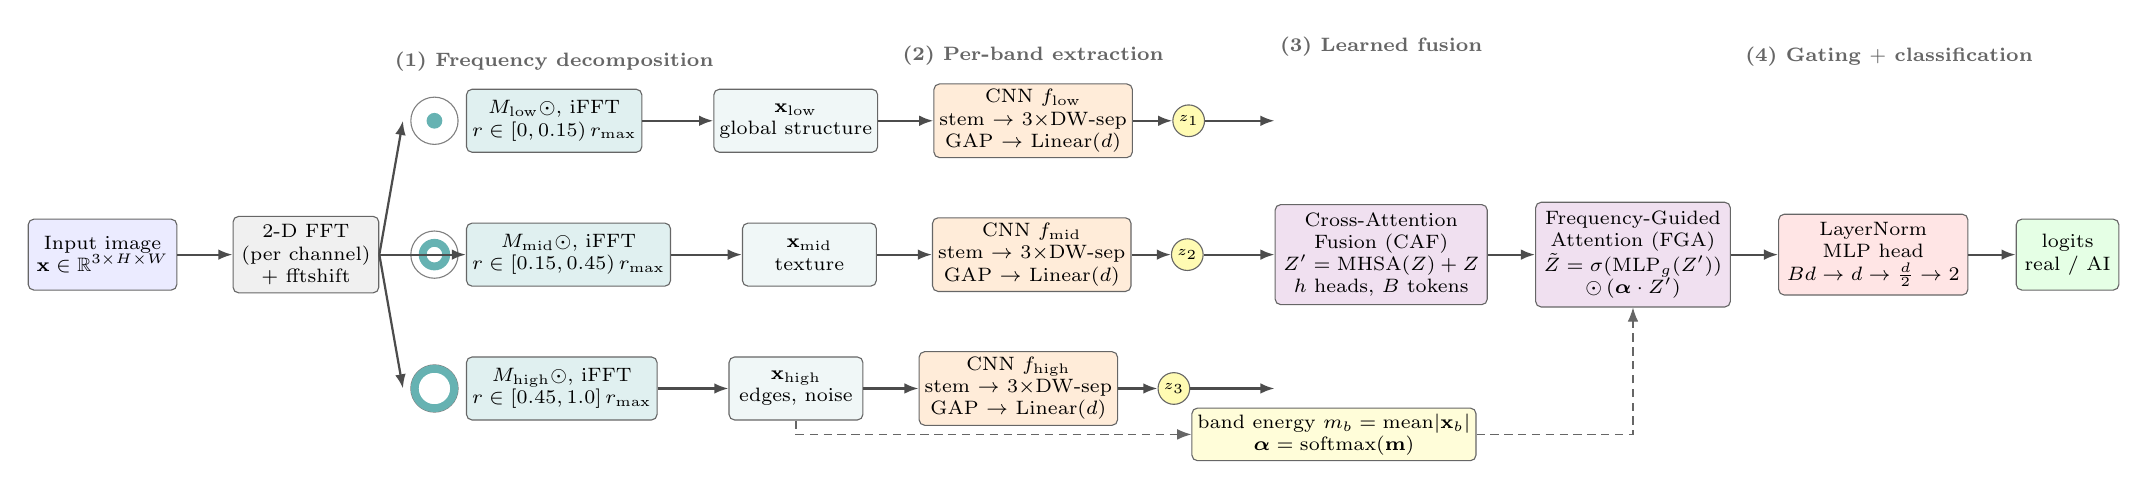
\begin{tikzpicture}[
  font=\scriptsize,
  node distance=4mm and 6mm,
  block/.style={draw=black!60, rounded corners=2pt, fill=blue!8,
                minimum height=9mm, align=center, inner sep=3pt},
  bandblk/.style={draw=black!60, rounded corners=2pt, fill=teal!12,
                minimum height=8mm, minimum width=17mm, align=center, inner sep=2pt},
  extblk/.style={draw=black!60, rounded corners=2pt, fill=orange!15,
                minimum height=8mm, align=center, inner sep=2pt},
  fuseblk/.style={draw=black!60, rounded corners=2pt, fill=violet!12,
                minimum height=10mm, align=center, inner sep=3pt},
  headblk/.style={draw=black!60, rounded corners=2pt, fill=red!10,
                minimum height=10mm, align=center, inner sep=3pt},
  tok/.style={draw=black!60, circle, fill=yellow!30, inner sep=1.2pt, font=\tiny},
  arr/.style={-{Latex[length=1.8mm]}, thick, black!70},
  darr/.style={-{Latex[length=1.8mm]}, densely dashed, black!60},
  stage/.style={font=\bfseries\scriptsize, text=black!60}
]
% ---- input and FFT ----
\node[block, minimum width=17mm] (input)
  {Input image\\ $\mathbf{x}\in\mathbb{R}^{3\times H\times W}$};
\node[block, right=7mm of input, fill=gray!12] (fft)
  {2-D FFT\\ (per channel)\\ $+$ fftshift};

% ---- three mask+band rows ----
\node[bandblk, right=11mm of fft, yshift=17mm] (mlow)
  {$M_{\mathrm{low}}\odot$, iFFT\\ $r\in[0,0.15)\,r_{\max}$};
\node[bandblk, right=11mm of fft] (mmid)
  {$M_{\mathrm{mid}}\odot$, iFFT\\ $r\in[0.15,0.45)\,r_{\max}$};
\node[bandblk, right=11mm of fft, yshift=-17mm] (mhigh)
  {$M_{\mathrm{high}}\odot$, iFFT\\ $r\in[0.45,1.0]\,r_{\max}$};

% annulus icons to the left of each mask block
\foreach \n/\ri/\ro in {mlow/0.0/0.10, mmid/0.10/0.20, mhigh/0.20/0.30}{
  \begin{scope}
    \coordinate (c\n) at ($(\n.west)+(-4mm,0)$);
    \draw[black!50] (c\n) circle (0.30);
    \ifdim \ri pt=0.0pt
      \fill[teal!60] (c\n) circle (\ro);
    \else
      \fill[teal!60, even odd rule] (c\n) circle (\ro) (c\n) circle (\ri);
    \fi
  \end{scope}
}

% ---- band images ----
\node[bandblk, right=9mm of mlow, fill=teal!6]  (blow)  {$\mathbf{x}_{\mathrm{low}}$\\ global structure};
\node[bandblk, right=9mm of mmid, fill=teal!6]  (bmid)  {$\mathbf{x}_{\mathrm{mid}}$\\ texture};
\node[bandblk, right=9mm of mhigh, fill=teal!6] (bhigh) {$\mathbf{x}_{\mathrm{high}}$\\ edges, noise};

% ---- extractors ----
\node[extblk, right=7mm of blow]  (elow)  {CNN $f_{\mathrm{low}}$\\ stem $\to$ 3$\times$DW-sep\\ GAP $\to$ Linear($d$)};
\node[extblk, right=7mm of bmid]  (emid)  {CNN $f_{\mathrm{mid}}$\\ stem $\to$ 3$\times$DW-sep\\ GAP $\to$ Linear($d$)};
\node[extblk, right=7mm of bhigh] (ehigh) {CNN $f_{\mathrm{high}}$\\ stem $\to$ 3$\times$DW-sep\\ GAP $\to$ Linear($d$)};

% ---- tokens ----
\node[tok, right=5mm of elow]  (t1) {$z_{1}$};
\node[tok, right=5mm of emid]  (t2) {$z_{2}$};
\node[tok, right=5mm of ehigh] (t3) {$z_{3}$};

% ---- fusion / FGA / head ----
\node[fuseblk, right=9mm of t2, minimum width=21mm] (caf)
  {Cross-Attention\\ Fusion (CAF)\\ $Z'=\mathrm{MHSA}(Z)+Z$\\ $h$ heads, $B$ tokens};
\node[fuseblk, right=6mm of caf, minimum width=21mm] (fga)
  {Frequency-Guided\\ Attention (FGA)\\ $\tilde{Z}=\sigma(\mathrm{MLP}_g(Z'))$\\ $\odot\,(\boldsymbol{\alpha}\cdot Z')$};
\node[headblk, right=6mm of fga, minimum width=19mm] (head)
  {LayerNorm\\ MLP head\\ $Bd \to d \to \frac{d}{2} \to 2$};
\node[block, right=6mm of head, fill=green!10, minimum width=13mm] (out)
  {logits\\ real / AI};

% ---- band-energy side path ----
\node[draw=black!60, rounded corners=2pt, fill=yellow!15, align=center,
      inner sep=2pt, below=13mm of caf, xshift=-6mm] (energy)
  {band energy $m_b=\mathrm{mean}|\mathbf{x}_b|$\\
   $\boldsymbol{\alpha}=\mathrm{softmax}(\mathbf{m})$};

% ---- arrows ----
\draw[arr] (input) -- (fft);
\draw[arr] (fft.east) -- ($(mlow.west)+(-8mm,0)$);
\draw[arr] (fft.east) -- (mmid.west);
\draw[arr] (fft.east) -- ($(mhigh.west)+(-8mm,0)$);
\draw[arr] (mlow) -- (blow);
\draw[arr] (mmid) -- (bmid);
\draw[arr] (mhigh) -- (bhigh);
\draw[arr] (blow) -- (elow);
\draw[arr] (bmid) -- (emid);
\draw[arr] (bhigh) -- (ehigh);
\draw[arr] (elow) -- (t1);
\draw[arr] (emid) -- (t2);
\draw[arr] (ehigh) -- (t3);
\draw[arr] (t1.east) -- (caf.west|-t1);
\draw[arr] (t2.east) -- (caf.west);
\draw[arr] (t3.east) -- (caf.west|-t3);
\draw[arr] (caf) -- (fga);
\draw[arr] (fga) -- (head);
\draw[arr] (head) -- (out);
\draw[darr] (bhigh.south) |- (energy.west);
\draw[darr] (energy.east) -| (fga.south);

% ---- stage labels ----
\node[stage, above=1mm of mlow] {(1) Frequency decomposition};
\node[stage, above=1mm of elow] {(2) Per-band extraction};
\node[stage] at ($(caf.north)+(0,20mm)$) {(3) Learned fusion};
\node[stage] at ($(head.north)+(2mm,20mm)$) {(4) Gating $+$ classification};
\end{tikzpicture}%
}
\caption{MFFT methodology (three-band configuration shown). The input is transformed to the frequency domain per RGB channel, split by radial band-pass masks $M_b$ (annulus icons indicate the pass region), and inverted to spatial band images $\mathbf{x}_b$. Weight-independent depthwise-separable CNNs $f_b$ embed each band into a token $z_b\in\mathbb{R}^d$. Multi-head cross-attention fuses the $B$ band tokens; Frequency-Guided Attention gates the fused tokens with the physically measured band-energy distribution $\boldsymbol{\alpha}$ (dashed path); an MLP head produces the two-class logits. The decomposition and $\boldsymbol{\alpha}$ contain no trainable parameters.}
\label{fig:arch}
\end{figure*}

\begin{figure}[!t]
\centering
\includegraphics[width=\linewidth]{figures_opt/fig1_frequency_decomposition.jpg}
\caption{Radial frequency decomposition of an input image into low (global structure), mid (texture), and high (fine detail and noise) bands. Each band image is a deterministic, independently reproducible function of the input.}
\label{fig:freq_decomp}
\end{figure}

\subsection{Frequency Decomposition}
\label{sec:decomp}
We compute the 2D discrete Fourier transform of each RGB channel of the input with orthonormal normalization:
\begin{equation}
X(u,v) = \frac{1}{\sqrt{HW}}\sum_{h=0}^{H-1} \sum_{w=0}^{W-1} x(h,w)\, e^{-2\pi i \left(\frac{uh}{H} + \frac{vw}{W}\right)},
\label{eq:dft}
\end{equation}
shift the DC component to the center, and apply binary radial masks
\begin{equation}
M_b(u,v) = \mathbb{1}\!\left[\, r_{\mathrm{lo}}^{(b)} \le r(u,v) < r_{\mathrm{hi}}^{(b)} \,\right],
\label{eq:mask}
\end{equation}
with $r(u,v) = \sqrt{(u-u_c)^2 + (v-v_c)^2}$, center $(u_c, v_c) = (H/2, W/2)$, and cutoffs relative to $r_{\max}=\min(H,W)/2$. The three-band configuration uses \textbf{Low} $[0, 0.15)$, \textbf{Mid} $[0.15, 0.45)$, \textbf{High} $[0.45, 1.0]$; the four-band configuration (used by MFFT-Large) partitions into $[0,0.1)$, $[0.1,0.3)$, $[0.3,0.6)$, $[0.6,1.0]$. The masked spectrum $\tilde{X}_b = X_{\mathrm{shifted}} \odot M_b$ is inverted per channel (inverse shift, inverse FFT, real part) to a 3-channel spatial band image:
\begin{equation}
\mathbf{x}_b = \mathcal{F}^{-1}\!\big(\mathcal{F}_{\mathrm{shift}}^{-1}(\tilde{X}_b)\big) \in \mathbb{R}^{3 \times H \times W}.
\label{eq:ifft}
\end{equation}
The module is non-parametric; masks are cached per input resolution, so the runtime cost is $B$ FFT/iFFT pairs per image (under 10\% of total inference time; Section~\ref{sec:efficiency}). The low band captures global structure and composition; the mid band captures texture-scale content where diffusion denoising signatures concentrate; the high band captures fine detail, edges, and noise where GAN upsampling artifacts and the absence of sensor noise are most visible. The band cutoffs were chosen to align with these qualitative regimes; the four-band alternative is evaluated in the ablation study (Section~\ref{sec:ablation}).

\textbf{Soft band masks.} Hard binary masks introduce ringing (Gibbs) artifacts at the band boundaries. As an extension we replace the indicator in \eqref{eq:mask} with a sigmoid transition of width $\tau = 0.02\, r_{\max}$:
\begin{equation}
M_b^{\mathrm{soft}}(u,v) = \sigma\!\left(\frac{r - r_{\mathrm{lo}}^{(b)}}{\tau}\right) \cdot \sigma\!\left(\frac{r_{\mathrm{hi}}^{(b)} - r}{\tau}\right),
\label{eq:softmask}
\end{equation}
which removes the hard information split while remaining non-parametric; its effect is measured in Section~\ref{sec:extensions}.

\subsection{Per-Band Feature Extraction}
\label{sec:extractor}
Each band uses an architecturally identical but weight-independent extractor $f_b$, allowing specialization to its band's statistics. Table~\ref{tab:extractor} details the layer structure. A $3\times3$ stem convolution (stride 2, 32 channels, BatchNorm, GELU) is followed by three stages of depthwise separable convolutions (each: $3\times3$ depthwise stride-2 convolution, $1\times1$ pointwise expansion, BatchNorm, GELU), global average pooling, and a linear projection to the token dimension $d$ with LayerNorm. Depthwise separability reduces per-stage parameters by roughly a factor of $k^2 C_{\mathrm{out}} / (k^2 + C_{\mathrm{out}})$ relative to standard convolutions, keeping each extractor at approximately 80K ($d{=}128$), 146K ($d{=}384$), or 245K ($d{=}768$) parameters.

\textbf{Pretrained extractors (extension).} To decouple architecture from initialization when comparing against ImageNet-pretrained baselines, a matched-pretraining variant replaces each $f_b$ with an ImageNet-pretrained MobileNetV3-Small trunk followed by the same pooling/projection head (4.63M parameters at Base scale); Section~\ref{sec:extensions} reports its pilot behavior.

\textbf{NPR high-band residual (extension).} Following the neighboring-pixel-relation insight of Tan \textit{et al.}~\cite{tan2024npr}, the highest band's extractor can additionally receive the resampling residual
\begin{equation}
\mathrm{NPR}(\mathbf{x}) = \mathbf{x} - \mathrm{Up}_{\times 2}\!\big(\mathrm{Down}_{\times 2}(\mathbf{x})\big),
\label{eq:npr}
\end{equation}
concatenated channel-wise to $\mathbf{x}_{\mathrm{high}}$, isolating the local interpolation traces that generator upsampling layers imprint.

\begin{table}[!t]
\renewcommand{\arraystretch}{1.2}
\caption{Per-band feature extractor ($d = 384$, Base scale, shown). DW = depthwise, PW = pointwise convolution.}
\label{tab:extractor}
\centering
\setlength{\tabcolsep}{4pt}
\begin{tabular}{llrr}
\toprule
Stage & Operation & Output ch. & Params \\
\midrule
Stem    & Conv $3{\times}3$, s2 + BN + GELU        & 32  & 928 \\
Block 1 & DW $3{\times}3$ s2 + PW $1{\times}1$ + BN + GELU & 64  & 2{,}464 \\
Block 2 & DW $3{\times}3$ s2 + PW $1{\times}1$ + BN + GELU & 128 & 9{,}024 \\
Block 3 & DW $3{\times}3$ s2 + PW $1{\times}1$ + BN + GELU & 256 & 34{,}432 \\
Pool    & AdaptiveAvgPool $\rightarrow 1{\times}1$  & 256 & 0 \\
Head    & Linear $256 \rightarrow d$ + LayerNorm    & $d$ & 99{,}456 \\
\midrule
\multicolumn{3}{l}{Total per extractor ($d=384$)} & $\approx$146K \\
\bottomrule
\end{tabular}
\end{table}

\subsection{Cross-Attention Fusion (CAF)}
\label{sec:caf}
Band embeddings $z_1,\dots,z_B \in \mathbb{R}^{d}$ are stacked into $Z \in \mathbb{R}^{B \times d}$ and passed through multi-head attention in which every band attends to every band:
\begin{align}
Q &= ZW_Q, \quad K = ZW_K, \quad V = ZW_V, \label{eq:qkv}\\
Z' &= \mathrm{Linear}\!\big(\mathrm{softmax}\!\big(QK^{\!\top}\!/\sqrt{d_k}\big)V\big) + Z, \label{eq:attn}
\end{align}
with $W_Q, W_K, W_V \in \mathbb{R}^{d \times d}$, $d_k = d/h$, and $h \in \{4, 6, 12\}$ heads for the Tiny/Base/Large variants. The residual connection preserves band-specific information while the attention path expresses input-dependent inter-band relationships. The motivating example is spectral consistency: natural images exhibit a characteristic power-law linking energy across bands, so \emph{anomalous high-frequency energy given the observed low-frequency structure} is evidence of synthesis---a relational cue that no single band and no element-wise fusion rule can represent. Table~\ref{tab:attnparams} gives the exact parameter accounting for the fusion and gating stages of each variant.

\begin{table}[!t]
\renewcommand{\arraystretch}{1.2}
\caption{Fusion and gating parameters by variant.}
\label{tab:attnparams}
\centering
\setlength{\tabcolsep}{3pt}
\begin{tabular}{lrrr}
\toprule
Component & Tiny ($d{=}128$) & Base ($d{=}384$) & Large ($d{=}768$) \\
\midrule
QKV projection   & 49{,}152  & 442{,}368 & 1{,}769{,}472 \\
Output projection& 16{,}512  & 147{,}840 & 590{,}592 \\
FGA gate MLP     & 8{,}384   & 74{,}208  & 295{,}872 \\
\bottomrule
\end{tabular}
\end{table}

\subsection{Frequency-Guided Attention (FGA)}
\label{sec:fga}
Standard attention weights are functions of learned projections and can exploit dataset-specific correlations---the semantic-shortcut failure mode documented for spatial detectors~\cite{shuai2026shortcuts}. FGA adds a weighting derived from a \emph{physical} property of the input that no learned prior can override. Let $m_b$ be the mean absolute magnitude of band image $\mathbf{x}_b$,
\begin{equation}
m_b = \frac{1}{CHW}\sum_{c,h,w} \left| x_b(c,h,w) \right|, \qquad \boldsymbol{\alpha} = \mathrm{softmax}(\mathbf{m}),
\label{eq:alpha}
\end{equation}
so $\boldsymbol{\alpha} \in \mathbb{R}^{B}$ measures where the input's spectral energy actually resides. FGA modulates the fused tokens as
\begin{equation}
\tilde{Z} = \sigma\!\big(\mathrm{MLP}_{\mathrm{gate}}(Z')\big) \odot \big(\boldsymbol{\alpha} \cdot Z'\big),
\label{eq:fga}
\end{equation}
combining the physics-derived band weighting with a learned per-feature gate ($d \rightarrow d/4 \rightarrow d$ bottleneck, ReLU, sigmoid). The intended benefit is robustness: on out-of-distribution inputs, learned attention may extrapolate arbitrarily, whereas $\boldsymbol{\alpha}$ remains a faithful summary of the input's spectrum. Whether this bias helps or constrains accuracy is an empirical question that our ablation addresses directly (Section~\ref{sec:ablation}).

\subsection{Classification Head and Training Objective}
The gated tokens are flattened to $\mathbb{R}^{B \cdot d}$, normalized (LayerNorm), and classified by a three-layer MLP: Linear $\rightarrow d$ (GELU, dropout 0.2), Linear $\rightarrow d/2$ (GELU, dropout 0.1), Linear $\rightarrow 2$. Head sizes are approximately 58K (Tiny), 519K (Base), and 2.66M (Large) parameters. We minimize cross-entropy with label smoothing $\epsilon = 0.1$:
\begin{equation}
\mathcal{L} = -\sum_{i=1}^N \sum_{c=1}^2 \left[(1-\epsilon)\,\delta_{y_i,c} + \tfrac{\epsilon}{2}\right] \log p_c(\mathbf{x}_i).
\label{eq:loss}
\end{equation}
Weights are initialized with truncated normal (std 0.02). Algorithm~\ref{alg:train} summarizes the training procedure.

\begin{algorithm}[!t]
\caption{MFFT forward pass}
\label{alg:forward}
\begin{algorithmic}[1]
\REQUIRE image $\mathbf{x}\in\mathbb{R}^{3\times H\times W}$; bands $\{(r_{\mathrm{lo}}^{(b)}, r_{\mathrm{hi}}^{(b)})\}_{b=1}^{B}$; extractors $\{f_b\}$; CAF, FGA, head parameters
\ENSURE logits $\hat{y}\in\mathbb{R}^{2}$
\STATE $X \leftarrow \mathrm{fftshift}(\mathrm{FFT2}(\mathbf{x}))$ \COMMENT{per RGB channel, Eq.~\eqref{eq:dft}}
\FOR{$b = 1$ \TO $B$}
    \STATE $M_b \leftarrow$ radial mask via Eq.~\eqref{eq:mask} (cached per resolution)
    \STATE $\mathbf{x}_b \leftarrow \Re\big[\mathrm{iFFT2}(\mathrm{ifftshift}(X \odot M_b))\big]$ \COMMENT{Eq.~\eqref{eq:ifft}}
    \STATE $z_b \leftarrow f_b(\mathbf{x}_b)$ \COMMENT{depthwise-separable CNN $\to \mathbb{R}^d$}
    \STATE $m_b \leftarrow \mathrm{mean}\,|\mathbf{x}_b|$ \COMMENT{band energy, Eq.~\eqref{eq:alpha}}
\ENDFOR
\STATE $Z \leftarrow \mathrm{stack}(z_1,\dots,z_B) \in \mathbb{R}^{B\times d}$
\STATE $Z' \leftarrow \mathrm{MHSA}(Z) + Z$ \COMMENT{cross-attention fusion, Eq.~\eqref{eq:attn}}
\STATE $\boldsymbol{\alpha} \leftarrow \mathrm{softmax}(m_1,\dots,m_B)$
\STATE $\tilde{Z} \leftarrow \sigma(\mathrm{MLP}_{\mathrm{gate}}(Z')) \odot (\boldsymbol{\alpha}\cdot Z')$ \COMMENT{FGA, Eq.~\eqref{eq:fga}}
\STATE $\hat{y} \leftarrow \mathrm{MLP}_{\mathrm{head}}(\mathrm{LayerNorm}(\mathrm{flatten}(\tilde{Z})))$
\RETURN $\hat{y}$
\end{algorithmic}
\end{algorithm}

\begin{algorithm}[!t]
\caption{MFFT training procedure (pilot protocol)}
\label{alg:train}
\begin{algorithmic}[1]
\REQUIRE training set $\mathcal{D}$, epochs $E$, batch size $m$, learning rate $\eta_0$, weight decay $\lambda$, label smoothing $\epsilon$
\STATE initialize all weights $\sim$ trunc.\ normal(0, $0.02$)
\STATE optimizer $\leftarrow$ AdamW($\eta_0{=}3{\times}10^{-4}$, $\lambda{=}0.05$)
\FOR{epoch $= 1$ \TO $E$}
    \FOR{minibatch $(\mathbf{x}, y) \sim \mathcal{D}$}
        \STATE $\mathbf{x} \leftarrow \mathrm{Augment}(\mathbf{x})$ \COMMENT{crop, flip, rotation, jitter, erasing}
        \STATE $\hat{y} \leftarrow$ Algorithm~\ref{alg:forward}$(\mathbf{x})$
        \STATE $\mathcal{L} \leftarrow$ label-smoothed cross-entropy, Eq.~\eqref{eq:loss}
        \STATE $g \leftarrow \nabla\mathcal{L}$; clip $\|g\|_2 \le 1.0$
        \STATE update weights; step warmup--cosine LR schedule
    \ENDFOR
    \STATE evaluate on validation split; checkpoint if best accuracy
\ENDFOR
\RETURN best checkpoint
\end{algorithmic}
\end{algorithm}

\subsection{Model Variants and Complexity}
\begin{table}[!t]
\renewcommand{\arraystretch}{1.2}
\caption{MFFT variants (pilot configuration, $224\times224$ input). Parameter counts and checkpoint sizes are measured, not estimated.}
\label{tab:variants}
\centering
\begin{tabular}{lccccc}
\toprule
Variant & $d$ & Heads & Bands & Params & Checkpoint \\
\midrule
MFFT-Tiny  & 128 & 4  & 3 & 372{,}450   & 1.5 MB \\
MFFT-Base  & 384 & 6  & 3 & 1{,}622{,}690 & 6.5 MB \\
MFFT-Large & 768 & 12 & 4 & 6{,}301{,}250 & 25.3 MB \\
\bottomrule
\end{tabular}
\end{table}
Table~\ref{tab:variants} lists the three variants. Tiny and Base use the three-band decomposition; Large scales both the token dimension and the band count, using the four-band partition. The per-image cost decomposes as
\begin{equation}
\underbrace{O\!\big(B\, HW \log HW\big)}_{\text{FFT/iFFT pairs}} +
\underbrace{O\!\big(B \sum_{\ell} H_\ell W_\ell k^2 C_\ell\big)}_{\text{band extractors}} +
\underbrace{O\!\big(B^2 d\big)}_{\text{attention}},
\label{eq:complexity}
\end{equation}
and because attention operates over only $B \in \{3,4\}$ tokens its cost is negligible; total compute is dominated by the per-band CNN extractors and the FFT pairs. Tiny targets edge and mobile deployment, Base standard servers, Large maximum accuracy.

% ============================================================
\section{Experimental Setup}
\label{sec:setup}
% ============================================================

\subsection{Corpus}
\label{sec:dataset}
We assembled a corpus of 2{,}696{,}760 images with a verified metadata manifest recording identifier, path, label, source, generator, dimensions, file size, and MD5 hash for every image. Table~\ref{tab:corpus} reports the exact composition, computed directly from the manifest. Real photographs (1.96M) come from Places365, ImageNet, the Pexels/Unsplash/Pixabay photography APIs, and Open Images V7. AI-generated images (608K) come from six generator sources: BigGAN (324K, including the GenImage~\cite{zhu2023genimage} subset), GLIDE (162K), Stable Diffusion (100K), DALL-E~3 (19K), and Midjourney (3.1K). Manipulated (deepfake) content (125K) comes from Celeb-DF~V2~\cite{li2020celebdf}, FaceForensics++~\cite{rossler2019}, and DFDC~\cite{dolhansky2020}. Zero-byte and corrupt files are filtered at manifest construction; 562 exact duplicates were removed by hash.

We note two properties relevant to the full-scale design. First, the corpus is class-imbalanced (72.8\% real), so full-scale training will use balanced sampling or reweighting; the pilot sidesteps the issue by drawing a balanced subset. Second, generator diversity is currently concentrated in GAN (BigGAN) and early-diffusion (GLIDE, SD) families; the remaining GenImage families (ADM, VQDM, Wukong, Midjourney at scale) and newer rectified-flow samplers (SDXL, SD3, FLUX)~\cite{esser2024} are being integrated so that leave-one-generator-out evaluation covers the full protocol.

\begin{table}[!t]
\renewcommand{\arraystretch}{1.2}
\caption{Corpus composition (from the verified manifest of 2{,}696{,}760 images).}
\label{tab:corpus}
\centering
\setlength{\tabcolsep}{4pt}
\begin{tabular}{llr}
\toprule
Class & Source / Generator & Images \\
\midrule
\multirow{4}{*}{Real (1{,}963{,}561)}
 & Places365            & 1{,}839{,}960 \\
 & ImageNet             & 98{,}001 \\
 & Pexels/Unsplash/Pixabay & 25{,}000 \\
 & Open Images V7       & 600 \\
\midrule
\multirow{5}{*}{AI-generated (608{,}072)}
 & BigGAN (incl.\ GenImage) & 323{,}995 \\
 & GLIDE                & 162{,}000 \\
 & Stable Diffusion     & 100{,}000 \\
 & DALL-E 3             & 18{,}998 \\
 & Midjourney           & 3{,}079 \\
\midrule
\multirow{3}{*}{Deepfake (125{,}127)}
 & Celeb-DF V2          & 101{,}031 \\
 & FaceForensics++      & 20{,}351 \\
 & DFDC                 & 3{,}745 \\
\bottomrule
\end{tabular}
\end{table}

\subsection{Pilot Protocol}
\label{sec:pilot}
From the corpus we drew a class-balanced subset of 5{,}000 images (2{,}500 real / 2{,}500 AI, where the AI class mixes fully generated and manipulated content) with a stratified 80/10/10 split (Table~\ref{tab:split}). All thirteen models train for \textbf{one epoch} at $224\times224$ under identical conditions. The single-epoch budget is a deliberate control: it equalizes compute across models and tests which architectures extract signal fastest from limited gradient steps, while acknowledging that pretrained baselines retain an advantage from their initialization. Table~\ref{tab:hyper} lists the complete hyperparameter set.

\begin{table}[!t]
\renewcommand{\arraystretch}{1.2}
\caption{Pilot data split (balanced subset of the corpus).}
\label{tab:split}
\centering
\begin{tabular}{lrrrr}
\toprule
Split & Total & Real & AI & Fraction \\
\midrule
Train      & 4{,}000 & 2{,}000 & 2{,}000 & 80\% \\
Validation & 500     & 250     & 250     & 10\% \\
Test       & 500     & 250     & 250     & 10\% \\
\midrule
Full pilot subset & 5{,}000 & 2{,}500 & 2{,}500 & 100\% \\
\bottomrule
\end{tabular}
\end{table}

\begin{table}[!t]
\renewcommand{\arraystretch}{1.15}
\caption{Training configuration (identical for all models).}
\label{tab:hyper}
\centering
\setlength{\tabcolsep}{4pt}
\begin{tabular}{ll}
\toprule
Hyperparameter & Value \\
\midrule
Optimizer & AdamW ($\beta_1{=}0.9$, $\beta_2{=}0.999$) \\
Learning rate & $3\times10^{-4}$ \\
Weight decay & 0.05 \\
Batch size (effective) & 32 \\
Warmup & 500 steps, linear from $0.01\times$ \\
Schedule & Cosine annealing w/ warm restarts \\
Gradient clipping & max-norm 1.0 \\
Label smoothing & $\epsilon = 0.1$ \\
Input resolution & $224\times224$ (pilot) \\
Epochs & 1 (pilot) \\
\midrule
\multicolumn{2}{l}{\textit{Augmentations (train)}} \\
Random resized crop & scale 0.85--1.0 \\
Horizontal flip & $p = 0.5$ \\
Rotation & $\pm 10^{\circ}$ \\
Color jitter & b/c/s 0.1, hue 0.05 \\
Random sharpness & factor 0.5--1.5, $p{=}0.3$ \\
Random erasing & $p = 0.25$ \\
Normalization & ImageNet mean/std \\
\midrule
\multicolumn{2}{l}{\textit{Preprocessing (eval)}} \\
Resize + center crop & to input resolution \\
\bottomrule
\end{tabular}
\end{table}

\subsection{Baselines}
\label{sec:baselines}
Ten baselines cover the main detector families under the identical pilot protocol; Table~\ref{tab:baseline_overview} summarizes them. \textbf{From scratch:} SimpleCNN, a five-stage plain CNN (Conv-BN-GELU, stride 2) with a small MLP head; LightViT, a compact ViT trained from random initialization; DeiT-S~\cite{touvron2021} (from scratch, isolating the architecture from its usual distillation recipe); and FreqDetect, our re-implementation of radial-spectrum classification after Frank \textit{et al.}~\cite{frank2020}---16 radial FFT magnitude bins per channel (48 features) classified by a three-layer MLP. \textbf{ImageNet-pretrained:} ResNet-18/50~\cite{he2016}, EfficientNet-B0~\cite{tan2019}, Swin-T~\cite{liu2021}, and ViT-B/16~\cite{dosovitskiy2021}, each with the classifier head replaced and the full network fine-tuned. \textbf{Foundation-model probe:} a linear probe on frozen CLIP ViT-B features~\cite{radford2021}, following the UnivFD recipe~\cite{ojha2023}. Appendix~\ref{app:baselines} gives implementation details.

\begin{table}[!t]
\renewcommand{\arraystretch}{1.2}
\caption{Baseline overview.}
\label{tab:baseline_overview}
\centering
\setlength{\tabcolsep}{4pt}
\begin{tabular}{llrl}
\toprule
Method & Family & Params & Initialization \\
\midrule
SimpleCNN   & plain CNN        & 422K   & random \\
LightViT    & compact ViT      & 2.04M  & random \\
DeiT-S~\cite{touvron2021} & ViT & 21.8M & random \\
FreqDetect~\cite{frank2020} & spectral + MLP & 14.7K & random \\
ResNet-18~\cite{he2016}   & CNN & 11.2M & ImageNet-1K \\
ResNet-50~\cite{he2016}   & CNN & 23.5M & ImageNet-1K \\
EfficientNet-B0~\cite{tan2019} & CNN & 4.0M & ImageNet-1K \\
Swin-T~\cite{liu2021}     & hierarchical ViT & 27.5M & ImageNet-1K \\
ViT-B/16~\cite{dosovitskiy2021} & ViT & 86.1M & ImageNet-1K \\
CLIP+Linear~\cite{radford2021,ojha2023} & frozen VLM + probe & 87.9M & LAION \\
\bottomrule
\end{tabular}
\end{table}

\subsection{Evaluation Metrics}
\label{sec:metrics}
On the held-out test split we report accuracy, precision, recall, and F1 with the AI class as positive:
\begin{equation}
\mathrm{Prec} = \frac{TP}{TP+FP},\;\;
\mathrm{Rec} = \frac{TP}{TP+FN},\;\;
F_1 = \frac{2\,\mathrm{Prec}\,\mathrm{Rec}}{\mathrm{Prec} + \mathrm{Rec}},
\label{eq:prf}
\end{equation}
together with AUC-ROC computed from the predicted class-probability scores. Calibration is assessed by the expected calibration error over 10 equal-width confidence bins,
\begin{equation}
\mathrm{ECE} = \sum_{k=1}^{10} \frac{|B_k|}{N}\, \big| \mathrm{acc}(B_k) - \mathrm{conf}(B_k) \big|,
\label{eq:ece}
\end{equation}
and by the Brier score $\frac{1}{N}\sum_i (p_i - y_i)^2$. For post-hoc calibration we apply temperature scaling~\cite{guo2017}: a scalar $T > 0$ fitted on the validation split by minimizing negative log-likelihood of the rescaled probabilities
\begin{equation}
p_c^{(T)}(\mathbf{x}) = \frac{\exp(\ell_c / T)}{\sum_{c'} \exp(\ell_{c'} / T)},
\label{eq:temp}
\end{equation}
where $\ell_c$ are the logits. Statistical uncertainty is quantified by nonparametric bootstrap 95\% confidence intervals (1{,}000 resamples of the test split), and paired model comparisons use the continuity-corrected McNemar test on the disagreement counts $n_{01}$ (only model A correct) and $n_{10}$ (only model B correct):
\begin{equation}
\chi^2 = \frac{\big(|n_{01} - n_{10}| - 1\big)^2}{n_{01} + n_{10}}.
\label{eq:mcnemar}
\end{equation}

\subsection{Leave-One-Generator-Out Protocol}
\label{sec:logoprotocol}
Following the cross-generator standard established by GenImage~\cite{zhu2023genimage} and reinforced by the 2025 audits~\cite{yan2025sanity,li2025aigibench}, we implement a leave-one-generator-out (LOGO) protocol (Algorithm~\ref{alg:logo}): for each generator family $g$ among \{BigGAN, GLIDE, Stable Diffusion, DALL-E~3, Midjourney, Celeb-DF, FaceForensics++, DFDC\}, a detector is trained on a balanced subset drawn from all fake sources \emph{except} $g$ (plus real images), then evaluated on held-out fakes from $g$ together with real images unseen during training. We report held-out fake accuracy, unseen-real accuracy, their balanced mean, and AUC.

\begin{algorithm}[!t]
\caption{Leave-one-generator-out (LOGO) evaluation}
\label{alg:logo}
\begin{algorithmic}[1]
\REQUIRE generator families $\mathcal{G}$; corpus manifest $\mathcal{M}$; budget $n$
\FOR{each held-out family $g \in \mathcal{G}$}
    \STATE $\mathcal{D}_{\mathrm{train}} \leftarrow$ balanced sample of $n$ images from $\mathcal{M}$ with fakes drawn from $\mathcal{G} \setminus \{g\}$ and reals from all real sources
    \STATE train MFFT-Base on $\mathcal{D}_{\mathrm{train}}$ (Algorithm~\ref{alg:train})
    \STATE $\mathcal{D}_{\mathrm{test}} \leftarrow$ held-out fakes of $g$ $\cup$ unseen real images
    \STATE record fake accuracy, real accuracy, balanced accuracy, AUC on $\mathcal{D}_{\mathrm{test}}$
\ENDFOR
\RETURN per-family table and mean balanced accuracy
\end{algorithmic}
\end{algorithm}

% ============================================================
\section{Pilot Results}
\label{sec:results}
% ============================================================

\subsection{Main Comparison}
\label{sec:main}
Table~\ref{tab:main} presents the pilot comparison, grouped by initialization---the variable that dominates a 1-epoch experiment. Three findings follow.

\begin{table}[!t]
\renewcommand{\arraystretch}{1.2}
\caption{Pilot comparison (1 epoch, 5K subset, $224\times224$). $^\dagger$trained from scratch; $^{*}$ImageNet/LAION-pretrained. Best per group in bold.}
\label{tab:main}
\centering
\setlength{\tabcolsep}{3.5pt}
\begin{tabular}{lrccccc}
\toprule
Method & Params & Acc. & Prec. & Rec. & F1 & AUC \\
\midrule
SimpleCNN$^\dagger$      & 422K   & 77.2 & 74.8 & 82.0 & 78.2 & 0.845 \\
LightViT$^\dagger$       & 2.04M  & 50.8 & 50.5 & 85.6 & 63.5 & 0.591 \\
DeiT-S$^\dagger$~\cite{touvron2021} & 21.8M  & 52.6 & 51.5 & 88.0 & 65.0 & 0.627 \\
FreqDetect$^\dagger$~\cite{frank2020} & 14.7K & 50.0 & 50.0 & 100.0 & 66.7 & 0.534 \\
\midrule
ResNet-18$^{*}$~\cite{he2016}    & 11.2M  & 96.0 & 94.6 & 97.6 & 96.1 & 0.991 \\
ResNet-50$^{*}$~\cite{he2016}    & 23.5M  & 97.2 & 96.8 & 97.6 & 97.2 & 0.998 \\
EfficientNet-B0$^{*}$~\cite{tan2019} & 4.0M & \textbf{98.2} & 99.2 & 97.2 & 98.2 & 1.000 \\
Swin-T$^{*}$~\cite{liu2021}      & 27.5M  & 95.2 & 96.3 & 94.0 & 95.1 & 0.992 \\
ViT-B/16$^{*}$~\cite{dosovitskiy2021} & 86.1M & 54.8 & 81.6 & 12.4 & 21.5 & 0.622 \\
CLIP+Linear$^{*}$~\cite{radford2021} & 87.9M & 66.8 & 78.4 & 46.4 & 58.3 & 0.765 \\
\midrule
MFFT-Tiny$^\dagger$  & 372K  & 81.6 & 75.5 & 93.6 & 83.6 & 0.931 \\
MFFT-Base$^\dagger$  & 1.62M & 88.6 & 92.1 & 84.4 & 88.1 & 0.939 \\
MFFT-Large$^\dagger$ & 6.30M & \textbf{91.4} & 87.9 & 96.0 & 91.8 & 0.964 \\
\bottomrule
\end{tabular}
\end{table}

\textbf{(1) Among from-scratch models, MFFT wins decisively.} MFFT-Large (91.4\%, 0.964 AUC) leads the best from-scratch competitor (SimpleCNN, 77.2\%) by 14.2 points; even MFFT-Tiny (372K parameters) beats SimpleCNN by 4.4 points with 12\% fewer parameters. Attention-only models without pretraining collapse in this regime---LightViT (50.8\%) and DeiT-S (52.6\%) barely exceed chance---confirming the known data hunger of transformers lacking either pretraining or a strong inductive bias. MFFT contains attention yet avoids the collapse because attention operates over only three frequency-band tokens whose representations are produced by convolutional extractors; the frequency decomposition supplies the inductive bias that raw ViTs lack. The hand-crafted spectral baseline (FreqDetect) degenerates to always-positive prediction (recall 100\%, precision 50\%): aggregate radial statistics that separated GAN images from real ones in 2020 do not separate our mixed GAN/diffusion/deepfake class, underlining that \emph{learned, spatially-resolved} band representations---not spectral features per se---are what carries MFFT.

\textbf{(2) Pretrained CNNs lead the pilot, as expected.} EfficientNet-B0 (98.2\%) and ResNet-50 (97.2\%) benefit from ImageNet initialization, an advantage one epoch of fine-tuning does not equalize. The pilot therefore cannot establish whether MFFT closes this gap at scale; that is the central question for the full-scale study, and the matched-pretraining MFFT variant (Section~\ref{sec:extensions}) exists precisely to decouple architecture from initialization. Notably, large pretrained \emph{transformers} do not dominate: ViT-B/16 (54.8\%) and CLIP linear probing (66.8\%) underperform badly with one epoch and 4K training images, consistent with their sample-inefficiency in low-shot fine-tuning.

\textbf{(3) MFFT extracts signal quickly.} Reaching 88--91\% from random initialization within a single epoch supports the design claim that explicit frequency decomposition accelerates learning by removing the burden of discovering spectral structure from data. Section~\ref{sec:dynamics} quantifies this against the spatial-only ablation.

\subsection{Training Dynamics}
\label{sec:dynamics}
Table~\ref{tab:dynamics} reports the single-epoch training trajectories of the three variants; Fig.~\ref{fig:training} plots the loss and accuracy progression for MFFT-Base. Two observations are noteworthy. First, all three variants converge to within a narrow validation-loss range (0.39--0.48) in one epoch, with no instability despite the from-scratch initialization---the warmup plus cosine schedule and gradient clipping suffice. Second, capacity translates into early accuracy monotonically at Base scale and above (Tiny 81.2\%, Base 88.2\%, Large 88.0\% validation), while the spatial-only ablation model reaches only 83.4\% validation accuracy under the identical budget (Table~\ref{tab:ablation}): at equal compute, the decomposition is worth roughly five validation points at Base scale.

\begin{table}[!t]
\renewcommand{\arraystretch}{1.2}
\caption{Single-epoch training dynamics of the MFFT variants.}
\label{tab:dynamics}
\centering
\setlength{\tabcolsep}{4pt}
\begin{tabular}{lcccc}
\toprule
Variant & Train loss & Val.\ loss & Train acc. & Val.\ acc. \\
\midrule
MFFT-Tiny  & 0.419  & 0.479 & 86.5 & 81.2 \\
MFFT-Base  & 0.427  & 0.393 & 86.2 & 88.2 \\
MFFT-Large & 0.436  & 0.422 & 85.7 & 88.0 \\
\bottomrule
\end{tabular}
\end{table}

\begin{figure}[!t]
\centering
\includegraphics[width=\linewidth]{result/test/base_model/fig/fig2_training_history.png}
\caption{Training history for MFFT-Base over the pilot epoch (loss and accuracy on train and validation splits).}
\label{fig:training}
\end{figure}

\subsection{Per-Variant Analysis}
\label{sec:variants}

\subsubsection{MFFT-Base}
On the 500-image test split, MFFT-Base attains 88.6\% accuracy, 92.1\% precision, 84.4\% recall, F1 88.1\%, and AUC 0.939. The confusion matrix (Fig.~\ref{fig:confusion_base}) shows TN=232, FP=18, FN=39, TP=211: a false-positive rate of 7.2\% on real images against a false-negative rate of 15.6\% on AI images. The FN:FP ratio of 2.2:1 reflects a conservative bias---ambiguous inputs are more often called real---which is the preferable error direction in settings where false accusations are costlier than missed detections. The ROC curve (Fig.~\ref{fig:roc_base}) and precision--recall curve (Fig.~\ref{fig:pr_base}) show usable operating points across the threshold range.

\begin{figure}[!t]
\centering
\includegraphics[width=\linewidth]{result/test/base_model/fig/fig3_confusion_matrix.png}
\caption{MFFT-Base confusion matrix on the pilot test split (500 images).}
\label{fig:confusion_base}
\end{figure}

\begin{figure}[!t]
\centering
\includegraphics[width=\linewidth]{result/test/base_model/fig/fig4_roc_curve.png}
\caption{MFFT-Base ROC curve (AUC = 0.939) on the pilot test split.}
\label{fig:roc_base}
\end{figure}

\begin{figure}[!t]
\centering
\includegraphics[width=\linewidth]{result/test/base_model/fig/fig5_pr_curve.png}
\caption{MFFT-Base precision--recall curve on the pilot test split.}
\label{fig:pr_base}
\end{figure}

\subsubsection{MFFT-Tiny}
MFFT-Tiny reaches 81.6\% accuracy with the opposite error profile (Fig.~\ref{fig:confusion_tiny}): TN=174, FP=76, FN=16, TP=234, i.e., recall 93.6\% at precision 75.5\%. The 372K-parameter model detects almost all AI images but over-flags real ones---at this capacity the extractors appear to learn ``any unusual frequency content $\Rightarrow$ AI'' without the finer discrimination needed to absorb natural high-frequency variation (foliage, fabric, sensor noise) into the real class. Its AUC of 0.931, close to Base's 0.939, indicates that the \emph{ranking} of samples is nearly as good and the gap is largely a threshold/sharpness effect; threshold tuning or temperature scaling could trade its recall surplus for precision.

\begin{figure}[!t]
\centering
\includegraphics[width=\linewidth]{result/test/tiny_model/fig/fig3_confusion_matrix.png}
\caption{MFFT-Tiny confusion matrix: high recall (93.6\%), low precision (75.5\%)---the capacity-limited variant over-predicts the AI class.}
\label{fig:confusion_tiny}
\end{figure}

\subsubsection{MFFT-Large}
MFFT-Large achieves the best from-scratch result: 91.4\% accuracy, AUC 0.964 (Fig.~\ref{fig:roc_large}), with confusion matrix TN=217, FP=33, FN=10, TP=240 (Fig.~\ref{fig:confusion_large})---recall 96.0\% while keeping precision at 87.9\%. Compared with Tiny, the added capacity converts 43 false positives into true negatives while \emph{also} recovering 6 false negatives: scale improves both error types, not merely the threshold. Compared with Base, Large trades 15 additional false positives for 29 fewer false negatives, sitting at a more recall-oriented operating point with higher overall accuracy.

\begin{figure}[!t]
\centering
\includegraphics[width=\linewidth]{result/test/large_model/fig/fig3_confusion_matrix.png}
\caption{MFFT-Large confusion matrix on the pilot test split.}
\label{fig:confusion_large}
\end{figure}

\begin{figure}[!t]
\centering
\includegraphics[width=\linewidth]{result/test/large_model/fig/fig4_roc_curve.png}
\caption{MFFT-Large ROC curve (AUC = 0.964), the best from-scratch result in the pilot.}
\label{fig:roc_large}
\end{figure}

\subsubsection{Per-Class and Per-Category Behavior}
Table~\ref{tab:perclass} consolidates per-class precision/recall/F1 for all variants, and Table~\ref{tab:percat} breaks test accuracy down by content category (real photographs; fully AI-generated; AI-altered composites, i.e., manipulated real images). Two patterns are consistent. First, fully AI-generated images are detected well by all variants (81--95\%), with the capacity-limited Tiny paradoxically strongest (94.7\%)---a direct consequence of its trigger-happy operating point. Second, AI-\emph{altered} composites are detected at 89--100\% across variants; manipulated images that splice synthetic content into a real photograph appear to produce strong frequency discontinuities at manipulation boundaries that all model scales can exploit. We caution that the AI-altered cell rests on 44 test samples, so the 100\% figures carry wide uncertainty and require confirmation at scale. Fig.~\ref{fig:category} visualizes the category breakdown for MFFT-Base.

\begin{table}[!t]
\renewcommand{\arraystretch}{1.2}
\caption{Per-class metrics on the pilot test split (250 per class).}
\label{tab:perclass}
\centering
\setlength{\tabcolsep}{4pt}
\begin{tabular}{llccc}
\toprule
Variant & Class & Prec. & Rec. & F1 \\
\midrule
\multirow{2}{*}{MFFT-Tiny}  & Real & 91.6 & 69.6 & 79.1 \\
                            & AI   & 75.5 & 93.6 & 83.6 \\
\midrule
\multirow{2}{*}{MFFT-Base}  & Real & 85.6 & 92.8 & 89.1 \\
                            & AI   & 92.1 & 84.4 & 88.1 \\
\midrule
\multirow{2}{*}{MFFT-Large} & Real & 95.6 & 86.8 & 91.0 \\
                            & AI   & 87.9 & 96.0 & 91.8 \\
\bottomrule
\end{tabular}
\end{table}

\begin{table}[!t]
\renewcommand{\arraystretch}{1.2}
\caption{Test accuracy by content category (category sizes: real 250, AI-generated 206, AI-altered 44).}
\label{tab:percat}
\centering
\setlength{\tabcolsep}{4pt}
\begin{tabular}{lccc}
\toprule
Variant & Real & AI-generated & AI-altered \\
\midrule
MFFT-Tiny  & 69.6 & 94.7 & 88.6 \\
MFFT-Base  & 92.8 & 81.1 & 100.0 \\
MFFT-Large & 86.8 & 95.2 & 100.0 \\
\bottomrule
\end{tabular}
\end{table}

\begin{figure}[!t]
\centering
\includegraphics[width=\linewidth]{result/test/base_model/fig/fig8_class_distribution.png}
\caption{Per-category test accuracy for MFFT-Base across real, AI-generated, and AI-altered content.}
\label{fig:category}
\end{figure}

\subsubsection{Calibration}
Table~\ref{tab:calibration} reports calibration metrics; Fig.~\ref{fig:calibration} shows the MFFT-Base reliability diagram. Base is the best calibrated (ECE 0.080, Brier 0.096)---reasonable for a single-epoch model---and Large achieves the lowest Brier score (0.069) at somewhat higher ECE (0.101). Tiny is markedly miscalibrated (ECE 0.145, Brier 0.133), consistent with its skewed operating point. For forensic deployment, calibrated probabilities matter as much as accuracy: an analyst acting on a ``0.9 confidence'' flag needs that number to mean 90\%. Section~\ref{sec:statprobes} demonstrates that temperature scaling (Eq.~\eqref{eq:temp}) halves the ECE at pilot scale.

\begin{table}[!t]
\renewcommand{\arraystretch}{1.2}
\caption{Calibration on the pilot test split.}
\label{tab:calibration}
\centering
\begin{tabular}{lcc}
\toprule
Variant & ECE & Brier \\
\midrule
MFFT-Tiny  & 0.145 & 0.133 \\
MFFT-Base  & 0.080 & 0.096 \\
MFFT-Large & 0.101 & 0.069 \\
\bottomrule
\end{tabular}
\end{table}

\begin{figure}[!t]
\centering
\includegraphics[width=\linewidth]{result/test/base_model/fig/fig13_calibration_curve.png}
\caption{Reliability diagram for MFFT-Base (ECE = 0.080, Brier = 0.096).}
\label{fig:calibration}
\end{figure}

\subsection{Ablation Studies}
\label{sec:ablation}
Table~\ref{tab:ablation} isolates each architectural component under the pilot protocol at Base scale, Table~\ref{tab:bands} varies the number of bands, and Fig.~\ref{fig:ablation} summarizes all configurations. The findings:

\begin{table}[!t]
\renewcommand{\arraystretch}{1.2}
\caption{Component ablation (pilot protocol; Base-scale extractors). Validation and test accuracy in \%.}
\label{tab:ablation}
\centering
\setlength{\tabcolsep}{3pt}
\begin{tabular}{lcccc}
\toprule
Configuration & Params & Val. & Test & $\Delta$ vs.\ spatial \\
\midrule
Spatial-only (no decomposition) & 958K  & 83.4 & 81.8 & --- \\
Low band only                   & 958K  & 72.2 & 62.6 & $-19.2$ \\
Mid band only                   & 958K  & 89.2 & 87.2 & $+5.4$ \\
High band only                  & 958K  & 89.6 & 88.8 & $+7.0$ \\
3 bands, concat fusion          & 958K  & 87.6 & 87.0 & $+5.2$ \\
3 bands, average fusion         & 958K  & 90.6 & 89.8 & $+8.0$ \\
3 bands, max fusion             & 958K  & 91.4 & \textbf{90.6} & $+8.8$ \\
3 bands, cross-attn (no FGA)    & 1.55M & 90.0 & 90.0 & $+8.2$ \\
Full MFFT-Base (CAF + FGA)      & 1.62M & 88.2 & 88.6 & $+6.8$ \\
\bottomrule
\end{tabular}
\end{table}

\begin{table}[!t]
\renewcommand{\arraystretch}{1.2}
\caption{Band-count ablation (pilot protocol). The 4-band row is architecturally identical to MFFT-Large; see text.}
\label{tab:bands}
\centering
\begin{tabular}{lccc}
\toprule
Bands & Partition & Params & Test acc. \\
\midrule
2 & low, high & 1.62M & 88.4 \\
3 & low, mid, high & 1.62M & \textbf{88.6} \\
4 & low, low-mid, mid-high, high & 6.30M & 85.0 \\
\bottomrule
\end{tabular}
\end{table}

\begin{figure}[!t]
\centering
\includegraphics[width=\linewidth]{result/test/ablation/ablation_summary.png}
\caption{Ablation summary across all configurations (validation and test accuracy). Frequency decomposition dominates; fusion strategy differences are second-order at pilot scale.}
\label{fig:ablation}
\end{figure}

\textbf{(1) Frequency decomposition is the dominant factor (RQ1: confirmed).} Every multi-band configuration beats the spatial-only baseline by 5.2--8.8 points at \emph{identical} parameter count (958K for all static-fusion rows), and even a single well-chosen band (high: 88.8\%; mid: 87.2\%) outperforms spatial-only (81.8\%). The gain cannot be attributed to capacity---it is the representation.

\textbf{(2) Band identity matters (RQ3: answered).} The low band alone (62.6\%) is 19 points \emph{below} the spatial baseline: global luminance structure not only lacks discriminative traces but actively misleads at this scale. The high band is strongest (88.8\%), consistent with GAN upsampling artifacts and missing sensor noise; the mid band is close behind (87.2\%), consistent with diffusion denoising signatures. That mid and high are individually strong yet their fusion is stronger still (90.0--90.6\%) confirms the bands carry complementary, not redundant, information.

\textbf{(3) The fusion paradox (RQ2: currently negative).} In the 1-epoch regime, parameter-free max pooling (90.6\%) edges out cross-attention (90.0\%), and adding FGA lowers accuracy to 88.6\%. We report this honestly rather than obscure it. Our working hypothesis is undertraining: CAF and FGA add 0.66M parameters whose benefit---modeling inter-band \emph{relationships}---requires more gradient steps to materialize than element-wise pooling, and the validation-vs-test pattern (max fusion: 91.4/90.6; CAF+FGA: 88.2/88.6) shows the attention path had not yet fit even the training distribution. The pilot cannot distinguish this hypothesis from the alternative that static fusion simply suffices; the full-scale study re-runs all configurations at 20 epochs to decide it, and if max fusion still wins, the honest engineering conclusion will be a simpler, cheaper final model.

\textbf{(4) Band count and a run-variance caveat.} At matched Base capacity, two bands (dropping mid) lose only 0.2 points relative to three, consistent with the high band dominating; we retain the mid band because diffusion-specific signatures concentrate there~\cite{corvi2023} and the pilot's generator mix under-represents modern diffusion models. The 4-band row requires care: it is architecturally identical to MFFT-Large ($d{=}768$, 6.30M parameters), so it confounds band count with capacity---and its 85.0\% here versus the same architecture's 91.4\% in Table~\ref{tab:main} comes from two independent 1-epoch runs, indicating substantial run-to-run variance in this regime. An independent replication of the full ablation grid in our pipeline-verification session confirmed this variance directly: the max-fusion configuration, best in Table~\ref{tab:ablation} at 90.6\%, measured 60.4\% in the replication run under a different random state. Single-epoch orderings among the closely spaced fusion strategies are therefore not stable, which is precisely why the full-scale study will report seed-controlled means and confidence intervals for every configuration.

\subsection{Architecture Extensions}
\label{sec:extensions}
Table~\ref{tab:extensions} evaluates the three extensions of Section~\ref{sec:method} under the pilot protocol; these rows come from the independent verification session, whose same-session MFFT-Base reference measured 85.8\% test accuracy. None of the extensions improves over the default model in the 1-epoch regime: soft masks come closest (83.6\%), the matched-pretraining variant reaches 81.0\% despite its ImageNet initialization (its MobileNetV3 trunks receive band-limited images far from the ImageNet distribution, so the initialization advantage does not transfer within one epoch), the NPR residual lands at 77.8\%, and combining all three degrades to 67.0\%. We include these results because they falsify the naive expectation that pretrained extractors would immediately dominate, and because they identify the extensions as full-scale hypotheses rather than free wins: each targets robustness or generalization properties (ringing suppression, initialization matching, upsampling-trace isolation) whose benefits the in-distribution 1-epoch pilot is structurally unable to reveal.

\begin{table}[!t]
\renewcommand{\arraystretch}{1.2}
\caption{Architecture-extension ablation (verification session, pilot protocol). Reference: same-session MFFT-Base, 85.8\%.}
\label{tab:extensions}
\centering
\setlength{\tabcolsep}{4pt}
\begin{tabular}{lrcc}
\toprule
Configuration & Params & Val. & Test \\
\midrule
MFFT-Base (default, same session) & 1.62M & --- & \textbf{85.8} \\
$+$ soft band masks (Eq.~\eqref{eq:softmask}) & 1.62M & 86.0 & 83.6 \\
$+$ pretrained extractors & 4.63M & 81.8 & 81.0 \\
$+$ NPR high-band residual (Eq.~\eqref{eq:npr}) & 1.62M & 78.6 & 77.8 \\
$+$ all three combined & 4.63M & 69.0 & 67.0 \\
\bottomrule
\end{tabular}
\end{table}

\subsection{Qualitative Analysis}
\label{sec:qualitative}
Fig.~\ref{fig:tsne} projects the fused band embeddings of the test split via t-SNE: after a single epoch, real and AI samples already form largely separated clusters, with the boundary region populated by the confusion-matrix errors. Fig.~\ref{fig:freq_response} plots the average spectral profiles that motivate the design---AI-generated images deviate from the natural power-law decay precisely in the mid/high ranges the ablation identifies as discriminative. Fig.~\ref{fig:heatmaps} shows per-band anomaly heatmaps: for a real photograph, high-band energy follows edges and texture as expected under natural image statistics, whereas AI-generated samples show spatially incoherent high-band energy or unnaturally smooth regions where texture should exist. Fig.~\ref{fig:samples} presents sample predictions with confidence scores, including representative errors: false positives cluster on heavily textured or heavily compressed real photographs, and false negatives on high-quality diffusion outputs with minimal high-frequency residue---the same failure modes reported for prior frequency methods~\cite{corvi2023,ricker2024}.

\begin{figure}[!t]
\centering
\includegraphics[width=\linewidth]{result/test/base_model/fig/fig11_tsne_embeddings.png}
\caption{t-SNE of MFFT-Base fused band embeddings on the test split after one epoch of training.}
\label{fig:tsne}
\end{figure}

\begin{figure}[!t]
\centering
\includegraphics[width=\linewidth]{result/test/base_model/fig/fig12_frequency_response.png}
\caption{Average frequency response of real versus AI-generated test images. Deviations from natural spectral decay concentrate in the mid and high bands.}
\label{fig:freq_response}
\end{figure}

\begin{figure}[!t]
\centering
\includegraphics[width=\linewidth]{figures_opt/fig7_anomaly_heatmaps.jpg}
\caption{Intrinsic per-band anomaly heatmaps. Heatmaps derive directly from band-limited image content, not from post-hoc gradients, and are independently reproducible from the input alone.}
\label{fig:heatmaps}
\end{figure}

\begin{figure}[!t]
\centering
\includegraphics[width=\linewidth]{figures_opt/fig6_sample_predictions.jpg}
\caption{Sample MFFT-Base predictions with confidence scores and ground truth, including representative false positives (textured/compressed real photos) and false negatives (high-quality diffusion outputs).}
\label{fig:samples}
\end{figure}

\subsection{Efficiency}
\label{sec:efficiency}
Table~\ref{tab:efficiency} relates accuracy to deployment cost. MFFT achieves its pilot accuracy at 372K--6.3M parameters and 1.5--25~MB checkpoints, versus 4--88M parameters for the pretrained baselines and $\sim$300M for CLIP-scale universal detectors~\cite{ojha2023,tan2025c2pclip}. MFFT-Large approaches ResNet-18's pilot accuracy (91.4 vs.\ 96.0) with 44\% fewer parameters \emph{and no pretraining}; MFFT-Tiny outperforms the similarly-sized SimpleCNN by 4.4 points. The FFT decomposition adds under 10\% to inference latency since masks are precomputed and the transform is $O(HW \log HW)$; attention cost is negligible at 3--4 band tokens (Eq.~\eqref{eq:complexity}). This footprint permits platform-scale screening and edge deployment where foundation-model detectors are impractical.

\begin{table}[!t]
\renewcommand{\arraystretch}{1.2}
\caption{Accuracy--efficiency comparison (from-scratch models).}
\label{tab:efficiency}
\centering
\setlength{\tabcolsep}{4pt}
\begin{tabular}{lrrc}
\toprule
Model & Params & Checkpoint & Test acc. \\
\midrule
FreqDetect~\cite{frank2020} & 14.7K & $<$0.1 MB & 50.0 \\
MFFT-Tiny   & 372K   & 1.5 MB  & 81.6 \\
SimpleCNN   & 422K   & 1.7 MB  & 77.2 \\
MFFT-Base   & 1.62M  & 6.5 MB  & 88.6 \\
LightViT    & 2.04M  & 8.2 MB  & 50.8 \\
MFFT-Large  & 6.30M  & 25.3 MB & 91.4 \\
DeiT-S~\cite{touvron2021} & 21.8M & 87 MB & 52.6 \\
\bottomrule
\end{tabular}
\end{table}

% ============================================================
\section{Generalization, Robustness, and Statistical Probes}
\label{sec:probes}
% ============================================================
The 2025--2026 evaluation standard for this field is unambiguous: in-distribution accuracy alone is insufficient~\cite{yan2025sanity,li2025aigibench}. This section exercises the three protocols that standard demands---cross-generator transfer, post-processing robustness, and statistical rigor---end to end at pilot scale. All experiments in this section were run in an independent pipeline-verification session under the same 1-epoch budget, with evaluation cells of 120--500 images; the numbers are therefore \emph{directional probes} that validate the protocol and register preliminary observations, not headline claims.

\subsection{Cross-Generator Transfer (LOGO)}
\label{sec:logo}
Table~\ref{tab:logo} reports the leave-one-generator-out results of Algorithm~\ref{alg:logo} for MFFT-Base across eight held-out families. The mean balanced accuracy is 78.9\% (mean AUC 0.849), but the per-family spread is the real finding.

\begin{table}[!t]
\renewcommand{\arraystretch}{1.2}
\caption{Leave-one-generator-out probes (MFFT-Base, 1 epoch per fold). Fake = accuracy on held-out generator's fakes; Real = accuracy on unseen real images; Bal.\ = balanced accuracy.}
\label{tab:logo}
\centering
\setlength{\tabcolsep}{3.5pt}
\begin{tabular}{lcccc}
\toprule
Held-out family & Fake & Real & Bal. & AUC \\
\midrule
BigGAN            & 50.4  & 98.4  & 74.4  & 0.824 \\
GLIDE             & 86.0  & 89.6  & 87.8  & 0.925 \\
Stable Diffusion  & 40.8  & 73.2  & 57.0  & 0.641 \\
DALL-E 3          & 44.3  & 84.8  & 64.6  & 0.778 \\
Midjourney        & 50.0  & 100.0 & 75.0  & 0.667 \\
Celeb-DF          & 97.6  & 67.6  & 82.6  & 0.964 \\
FaceForensics++   & 100.0 & 93.1  & 96.6  & 0.998 \\
DFDC              & 100.0 & 85.7  & 92.9  & 1.000 \\
\midrule
Mean              & 71.1  & 86.6  & 78.9  & 0.849 \\
\bottomrule
\end{tabular}
\end{table}

Three patterns emerge. \textbf{(1) Deepfake manipulations transfer almost perfectly.} With FaceForensics++, Celeb-DF, or DFDC held out, held-out fake detection reaches 97.6--100\%: the splicing discontinuities that face manipulation imprints are generator-agnostic frequency evidence, and a detector trained on \emph{other} manipulation families still finds them. \textbf{(2) GLIDE transfers well, but modern diffusion does not.} Held-out GLIDE fakes are caught at 86.0\%, yet held-out Stable Diffusion (40.8\%) and DALL-E~3 (44.3\%) fall below chance on the fake side---the detector trained without them has learned artifacts (dominated by the BigGAN/GLIDE mix) that latent-diffusion outputs do not exhibit. This mirrors exactly the GAN-to-diffusion transfer gap documented in the literature~\cite{corvi2023,ojha2023,zhu2023genimage} and quantifies, for our architecture and corpus, where additional generator diversity is needed most. \textbf{(3) Small cells are visibly noisy.} The Midjourney fold evaluates on only a handful of held-out fakes (the corpus contains just 3.1K Midjourney images), so its 50\%/100\% split carries little evidential weight. These probes establish that our LOGO machinery is correct and that the full-scale run's most important ingredient is the pending integration of the remaining GenImage families and rectified-flow generators.

\subsection{Robustness to Post-Processing}
\label{sec:robustness}
Real-world images arrive re-compressed, resized, and filtered by social-media pipelines---the conditions under which the AIGIBench audit found detectors most brittle~\cite{li2025aigibench}. Table~\ref{tab:robustness} reports MFFT-Base accuracy and AUC under a JPEG/downscale/blur grid (120-image probe set per condition).

\begin{table}[!t]
\renewcommand{\arraystretch}{1.2}
\caption{Post-processing robustness probes (MFFT-Base, $n{=}120$ per condition).}
\label{tab:robustness}
\centering
\setlength{\tabcolsep}{4pt}
\begin{tabular}{llcc}
\toprule
Perturbation & Level & Acc.\ (\%) & AUC \\
\midrule
None (clean)  & ---        & 80.8 & 0.904 \\
\midrule
\multirow{5}{*}{JPEG}
 & quality 95 & 81.7 & 0.901 \\
 & quality 80 & 80.8 & 0.903 \\
 & quality 60 & 82.5 & 0.930 \\
 & quality 40 & 80.0 & 0.910 \\
 & quality 30 & 82.5 & 0.924 \\
\midrule
\multirow{3}{*}{Downscale}
 & $0.75\times$ & 55.8 & 0.783 \\
 & $0.50\times$ & 49.2 & 0.634 \\
 & $0.25\times$ & 50.8 & 0.498 \\
\midrule
\multirow{3}{*}{Gaussian blur}
 & $\sigma = 0.5$ & 73.3 & 0.883 \\
 & $\sigma = 1.0$ & 50.0 & 0.712 \\
 & $\sigma = 2.0$ & 52.5 & 0.476 \\
\bottomrule
\end{tabular}
\end{table}

The dichotomy is sharp and mechanistically interpretable. \textbf{JPEG compression barely moves the needle} (80.0--82.5\% across quality 30--95, AUC $\ge$ 0.90 throughout): JPEG quantizes block-DCT coefficients but preserves the radial energy \emph{distribution} that MFFT's band statistics summarize, and the training pipeline already includes JPEG augmentation. \textbf{Downscaling and blur are destructive} (accuracy falls to chance at $0.5\times$ downscaling or $\sigma{=}1.0$ blur): both operations are low-pass filters that physically remove the high-band content carrying most of the discriminative signal (Table~\ref{tab:ablation}). This is a known and fundamental limitation of high-frequency forensic cues~\cite{wang2020,tan2024freqnet}, and it prescribes the remedy the full-scale run will apply---random downscale--upscale and blur \emph{training} augmentation~\cite{wang2020}, plus the mid/low-band pathways whose weighting CAF can in principle shift toward surviving bands when the high band is erased. Testing whether adaptive fusion actually confers this resilience (hypothesis H4, Section~\ref{sec:fullscale}) is one of the sharpest questions the full-scale study can answer, since it is exactly the scenario where input-adaptive band weighting should beat any fixed rule.

\subsection{Calibration and Statistical Rigor}
\label{sec:statprobes}
On the verification session's MFFT-Base checkpoint, temperature scaling (Eq.~\eqref{eq:temp}) fitted on the validation split ($T = 0.741$) halves the expected calibration error from 0.059 to 0.029 and improves the Brier score from 0.130 to 0.126---confirming that MFFT's residual miscalibration at pilot scale is a global confidence-scale effect that one scalar corrects, rather than a structural ranking failure. Bootstrap 95\% confidence intervals (1{,}000 resamples) for the same checkpoint are: accuracy 81.8\% [78.4, 84.8], precision 78.9\% [74.4, 83.5], recall 86.8\% [82.4, 90.8], F1 82.7\% [79.0, 85.9], AUC 0.912 [0.886, 0.936]. A paired McNemar test (Eq.~\eqref{eq:mcnemar}) between the Base and Tiny variants yields $n_{01}{=}42$, $n_{10}{=}53$, $\chi^2 = 1.05$, $p = 0.305$: at 500 test images the observed Base--Tiny gap is \emph{not} statistically significant, a sobering and useful demonstration of why the full-scale study's 270K-image test split is necessary before any between-model claim is made. All three procedures are scripted and will run unchanged at full scale.

% ============================================================
\section{Discussion}
\label{sec:discussion}
% ============================================================

\subsection{What the Pilot Establishes}
The pilot supports three of the five research questions. \textbf{RQ1 (confirmed):} explicit frequency decomposition improves detection over spatial-only processing by 5--9 points at identical parameter count and compute. \textbf{RQ3 (answered):} the discriminative signal resides in the mid and especially high bands; the low band alone is counterproductive. \textbf{RQ5 (supported):} among from-scratch models the architecture is decisively parameter-efficient---91.4\% at 6.3M parameters where plain CNNs reach 77\% and compact ViTs collapse. Two questions receive preliminary and partly negative answers. \textbf{RQ2 (currently negative):} learned cross-attention fusion does not yet beat max pooling, and single-epoch fusion orderings are unstable across runs; the full-scale study decides whether this is undertraining or a real ceiling. \textbf{RQ4 (probed):} the LOGO probes show a bimodal transfer profile---near-perfect on manipulation deepfakes and GLIDE, chance-level on held-out latent diffusion---and the robustness probes show JPEG stability alongside low-pass fragility. We consider stating these open questions explicitly to be a feature of this paper: they define exactly what the full-scale campaign must measure, with the hypotheses registered in advance (Section~\ref{sec:fullscale}).

\subsection{Why Multi-Band Analysis Should Generalize (Hypothesis)}
The mechanistic argument for multi-band robustness is that a generator may suppress artifacts in one band---modern GAN variants mitigate checkerboarding; diffusion models increasingly match natural spectra at low frequencies---but eliminating traces \emph{simultaneously across all bands} requires matching the full joint spectral distribution of natural images, which no current sampler achieves~\cite{corvi2023,ricker2024}. Cross-attention over bands can in principle exploit inter-band consistency (natural images exhibit characteristic spectral decay linking bands), a relational cue unavailable to single-band methods, and FGA anchors the fused representation to the input's physical spectrum, limiting the room for the semantic shortcuts that undermine spatial detectors in the wild~\cite{yan2025sanity,shuai2026shortcuts}. The LOGO probes neither confirm nor refute this yet: transfer succeeded where artifacts are strong and band-localized (manipulation boundaries, GLIDE upsampling) and failed where the training mix simply lacked the relevant artifact family (latent diffusion). The decisive test requires the diversified corpus.

\subsection{Interpreting the Fusion Paradox}
Three explanations are consistent with the pilot data. (a)~\emph{Undertraining}: relational weights need more gradient steps than element-wise pooling; the attention configurations' validation--test gap pattern supports this. (b)~\emph{Task simplicity at pilot scale}: with a generator mix dominated by BigGAN and GLIDE, whose artifacts are strong and band-localized, picking the loudest band (max pooling) may simply be optimal, and relational cues add nothing; a more diverse generator mix at full scale would then favor adaptive fusion. (c)~\emph{Over-regularization}: FGA's physics-derived $\boldsymbol{\alpha}$ weighting constrains the fused representation; if the constraint is misaligned with the task, it costs accuracy in-distribution but may still buy robustness out-of-distribution---measurable only with the full-scale robustness suite. The experimental design of Section~\ref{sec:fullscale} distinguishes (a) from (b)/(c) by re-running the ablation at 20 epochs, and (b) from (c) by comparing in-distribution and cross-generator deltas for the FGA and no-FGA models. The run-variance finding of Section~\ref{sec:ablation} adds a fourth consideration: at one epoch, some of the observed ordering is noise, and any resolution of the paradox must rest on seed-controlled statistics.

\subsection{Scaling Behavior Across Variants}
The three variants trace an informative capacity path. Tiny (372K) achieves high recall but poor precision and calibration---enough capacity to detect spectral anomalies, not enough to model the natural variability of real photographs. Base (1.62M) is the most balanced and best calibrated. Large (6.30M) improves both error types over Tiny and overall accuracy over Base, settling at a recall-oriented operating point (96.0\% recall at 87.9\% precision). The monotone AUC progression (0.931 $\rightarrow$ 0.939 $\rightarrow$ 0.964) indicates genuine representational gains with scale, not threshold artifacts. For deployment, this suggests: Tiny as a high-recall pre-filter whose flags are confirmed downstream; Base where calibrated probabilities matter; Large where accuracy dominates cost.

\subsection{Interpretability: Constitutive Versus Attributional Evidence}
\label{sec:interpretability}
Because band images are deterministic functions of the input (Section~\ref{sec:decomp}), the per-band heatmaps of Fig.~\ref{fig:heatmaps} constitute \emph{constitutive} evidence---an analyst can regenerate them with any FFT tool and verify the flagged anomaly exists in the image itself. Post-hoc saliency such as Grad-CAM~\cite{selvaraju2017} or integrated gradients~\cite{sundararajan2017} instead produces \emph{attributional} evidence---a statement about the model, subject to gradient saturation and attribution error, and unverifiable without model access. In forensic and journalistic workflows this distinction is material: constitutive evidence survives cross-examination that attributional evidence may not. Combined with calibrated confidence (Section~\ref{sec:statprobes}) and per-band FGA weights indicating \emph{which} spectral range drove a decision, MFFT supports a human-in-the-loop protocol in which the system's output is an inspectable evidence package rather than a bare score.

\subsection{Practical Implications}
For practitioners, the pilot suggests five guidelines. First, if a detector must be trained from scratch---for data-governance reasons, or for input modalities where no pretrained backbone exists---explicit frequency decomposition is the highest-leverage architectural choice we measured (+5 to +9 points at equal cost). Second, compact attention over a few semantically meaningful tokens (here, bands) avoids the data hunger of full patch-token ViTs. Third, calibration should be reported alongside accuracy, and temperature scaling is a nearly free improvement; our variants differ more in ECE than in AUC, and deployment consequences differ accordingly. Fourth, robustness evaluation must include low-pass perturbations, not only JPEG: our probes show a detector can look robust under the most commonly reported perturbation while failing under resizing that every social platform applies. Fifth, efficiency claims should be grounded in deployment artifacts (parameters, checkpoint size, latency overhead) rather than FLOPs alone; MFFT's 1.5--25~MB checkpoints permit on-device screening that 300M-parameter universal detectors cannot.

% ============================================================
\section{Limitations}
\label{sec:limitations}
% ============================================================
\begin{enumerate}
    \item \textbf{Pilot scale only.} All results are 1-epoch, 5K-subset, $224\times224$; absolute numbers will change at scale, and nothing here is a state-of-the-art comparison against the 2024--2026 systems of Section~\ref{sec:related}, which would require matched full-convergence training.
    \item \textbf{Directional generalization evidence only.} The LOGO and robustness probes use small evaluation cells (120--500 images; a handful for Midjourney) and 1-epoch folds; they validate protocol and reveal gross patterns, not fine rankings.
    \item \textbf{Initialization confound.} Comparisons against pretrained baselines conflate architecture with initialization; the matched-pretraining MFFT variant exists but itself needs more than one epoch for its initialization to matter.
    \item \textbf{Run-to-run variance.} Independent 1-epoch replications reorder the closely spaced fusion configurations (max fusion: 90.6\% vs.\ 60.4\%); conclusions about second-order design choices require seed-controlled repetition.
    \item \textbf{Small cells.} The AI-altered category has 44 test samples; its 100\% figures carry wide uncertainty.
    \item \textbf{The fusion paradox is unresolved.} The pilot ordering (max $>$ CAF $>$ CAF+FGA) contradicts the motivating hypothesis and must be settled at scale before the architecture is finalized.
    \item \textbf{Corpus skew.} The current generator mix over-represents BigGAN/GLIDE and under-represents modern latent-diffusion and rectified-flow samplers---exactly the families the LOGO probes identify as the transfer gap.
    \item \textbf{Design choices untested.} Binary radial masks with fixed cutoffs and the specific band partitions are pilot-validated but not optimized; learnable band boundaries are a planned extension. The band-count comparison additionally confounds band count with capacity.
\end{enumerate}

% ============================================================
\section{Planned Full-Scale Study}
\label{sec:fullscale}
% ============================================================
The forthcoming campaign on university DGX infrastructure will train all thirteen models for 20 epochs at $384\times384$ with mixed precision on the full corpus (stratified 80/10/10: $\sim$2.16M/270K/270K) using balanced sampling, and will add the components required for a complete evaluation:
\begin{enumerate}
    \item \textbf{Cross-generator hold-out (RQ4):} leave-one-generator-out over the GenImage families plus DALL-E~3 and Midjourney, following~\cite{zhu2023genimage}; mean cross-generator accuracy is the primary endpoint, with the SD/DALL-E~3 transfer gap of Table~\ref{tab:logo} as the pre-registered weak point to close.
    \item \textbf{Cross-dataset transfer:} evaluation on CIFAKE, the in-the-wild Chameleon set~\cite{yan2025sanity}, and the AIGIBench degradation tasks~\cite{li2025aigibench} without retraining.
    \item \textbf{Robustness suite:} the full JPEG/downscale/blur grid of Table~\ref{tab:robustness} at scale, with random JPEG, downscale--upscale, and blur added to training augmentation following~\cite{wang2020}.
    \item \textbf{Statistical rigor:} bootstrap 95\% confidence intervals on all headline metrics and McNemar tests against the strongest baseline, as demonstrated in Section~\ref{sec:statprobes}.
    \item \textbf{Matched-pretraining variant:} MFFT with ImageNet-pretrained band extractors at full convergence, decoupling architecture from initialization.
    \item \textbf{Full ablation re-run:} all thirteen configurations at 20 epochs over multiple seeds, pre-registering the fusion-paradox hypotheses.
    \item \textbf{Calibration:} temperature scaling on validation, reporting pre/post ECE for all models.
\end{enumerate}
Pre-registered hypotheses: \textbf{H1} --- the frequency-decomposition advantage over spatial-only persists at full training; \textbf{H2} --- CAF+FGA overtakes max pooling once trained to convergence on a diverse generator mix; \textbf{H3} --- MFFT's cross-generator degradation is smaller than that of spatial baselines of comparable or larger capacity; \textbf{H4} --- FGA improves robustness under post-processing even if in-distribution accuracy is unchanged. Outcomes will be reported for all four regardless of direction.

% ============================================================
\section{Ethical Considerations}
\label{sec:ethics}
% ============================================================
Detection systems for synthetic media carry dual-use and fairness risks. The intended use of MFFT is defensive: supporting journalists, fact-checkers, forensic analysts, and content-moderation teams. False positives risk wrongly discrediting authentic material---our conservative operating points and calibrated confidences are chosen to mitigate this, and we recommend human review of all flags. False negatives risk unwarranted trust; no detector output should be treated as proof. Publishing discriminative features could inform evasion; we judge the transparency and reproducibility benefits to outweigh this, consistent with community norms, and note that the underlying artifacts stem from generator architecture rather than from secrets our disclosure reveals. Detection accuracy may vary across demographic and cultural content distributions; the full-scale study's per-category analysis will report performance disaggregated by content type, and the corpus draws real photographs from geographically diverse sources. Code, manifests, and checkpoints will be released to enable independent auditing.

% ============================================================
\section{Conclusion}
\label{sec:conclusion}
% ============================================================
We presented MFFT, a compact multi-band frequency architecture for AI-generated image detection, with a complete design analysis, a controlled pilot validation, and an end-to-end demonstration of the generalization, robustness, and statistical protocols that current evaluation standards demand. The pilot delivers three verified findings: from scratch and at equal compute, explicit frequency decomposition improves detection by 5--9 points over spatial-only processing at identical parameter count; the discriminative signal concentrates in the mid and high frequency bands; and MFFT-Large leads all from-scratch models at 91.4\% accuracy (0.964 AUC) with 6.3M parameters and a 25~MB checkpoint, while MFFT-Base offers the best calibration (ECE 0.080, halved again by temperature scaling) at 1.6M parameters. The probes add two structural findings with full-scale consequences: cross-generator transfer is bimodal---near-perfect on manipulation deepfakes, chance-level on held-out latent diffusion---and robustness is JPEG-stable but low-pass-fragile. The paper also registers, in advance, the open questions the full-scale study must answer: whether learned cross-attention fusion overtakes simple pooling with adequate training, and whether frequency-guided gating buys out-of-distribution robustness. We release code, manifests, and checkpoints to make both the pilot and the forthcoming full-scale results reproducible.

% ============================================================
\begin{thebibliography}{60}

\bibitem{rombach2022} R.~Rombach, A.~Blattmann, D.~Lorenz, P.~Esser, and B.~Ommer, ``High-resolution image synthesis with latent diffusion models,'' in \textit{Proc. IEEE/CVF CVPR}, 2022, pp. 10684--10695.

\bibitem{esser2024} P.~Esser, S.~Kulal, A.~Blattmann, R.~Entezari, J.~M\"uller, H.~Saini, Y.~Levi, D.~Lorenz, A.~Sauer, F.~Boesel, D.~Podell, T.~Dockhorn, Z.~English, and R.~Rombach, ``Scaling rectified flow transformers for high-resolution image synthesis,'' in \textit{Proc. ICML}, 2024.

\bibitem{karras2019} T.~Karras, S.~Laine, and T.~Aila, ``A style-based generator architecture for generative adversarial networks,'' in \textit{Proc. IEEE/CVF CVPR}, 2019, pp. 4401--4410.

\bibitem{betker2023} J.~Betker \textit{et al.}, ``Improving image generation with better captions,'' OpenAI Tech. Rep., 2023.

\bibitem{wang2020} S.-Y.~Wang, O.~Wang, R.~Zhang, A.~Owens, and A.~A.~Efros, ``CNN-generated images are surprisingly easy to spot... for now,'' in \textit{Proc. IEEE/CVF CVPR}, 2020, pp. 8695--8704.

\bibitem{ojha2023} U.~Ojha, Y.~Li, and Y.~J.~Lee, ``Towards universal fake image detectors that generalize across generative models,'' in \textit{Proc. IEEE/CVF CVPR}, 2023, pp. 24480--24489.

\bibitem{zhu2023genimage} M.~Zhu \textit{et al.}, ``GenImage: A million-scale benchmark for detecting AI-generated image,'' in \textit{Proc. NeurIPS Datasets and Benchmarks}, 2023.

\bibitem{tan2024npr} C.~Tan, Y.~Zhao, S.~Wei, G.~Gu, P.~Liu, and Y.~Wei, ``Rethinking the up-sampling operations in CNN-based generative network for generalizable deepfake detection,'' in \textit{Proc. IEEE/CVF CVPR}, 2024, pp. 28130--28139.

\bibitem{corvi2023} R.~Corvi, D.~Cozzolino, G.~Zingarini, G.~Poggi, K.~Nagano, and L.~Verdoliva, ``On the detection of synthetic images generated by diffusion models,'' in \textit{Proc. IEEE ICASSP}, 2023.

\bibitem{yan2025sanity} S.~Yan, O.~Li, J.~Cai, Y.~Hao, X.~Jiang, Y.~Hu, and W.~Xie, ``A sanity check for AI-generated image detection,'' in \textit{Proc. ICLR}, 2025.

\bibitem{li2025aigibench} Z.~Li, J.~Yan, Z.~He, K.~Zeng, W.~Jiang, L.~Xiong, and Z.~Fu, ``Is artificial intelligence generated image detection a solved problem?'' arXiv:2505.12335, 2025.

\bibitem{shuai2026shortcuts} C.~Shuai, S.~Fan, C.~Zou, B.~Gong, W.~Lian, X.~Bi, Z.~Liu, Z.~Ba, and K.~Ren, ``When detectors forget forensics: Blocking semantic shortcuts for generalizable AI-generated image detection,'' arXiv:2603.09242, 2026.

\bibitem{zhang2019wifs} X.~Zhang, S.~Karaman, and S.-F.~Chang, ``Detecting and simulating artifacts in GAN fake images,'' in \textit{Proc. IEEE WIFS}, 2019.

\bibitem{durall2020} R.~Durall, M.~Keuper, and J.~Keuper, ``Watch your up-convolution: CNN based generative deep neural networks are failing to reproduce spectral distributions,'' in \textit{Proc. IEEE/CVF CVPR}, 2020, pp. 7890--7899.

\bibitem{frank2020} J.~Frank, T.~Eisenhofer, L.~Sch\"onherr, A.~Fischer, D.~Kolossa, and T.~Holz, ``Leveraging frequency analysis for deep fake image recognition,'' in \textit{Proc. ICML}, 2020, pp. 3247--3258.

\bibitem{cozzolino2019} D.~Cozzolino and L.~Verdoliva, ``Noiseprint: A CNN-based camera model fingerprint,'' \textit{IEEE Trans. Inf. Forensics Security}, vol.~15, pp. 144--159, 2019.

\bibitem{ricker2024} J.~Ricker, S.~Damm, T.~Holz, and A.~Fischer, ``Towards the detection of diffusion model deepfakes,'' in \textit{Proc. VISAPP}, 2024.

\bibitem{tan2024freqnet} C.~Tan, Y.~Zhao, S.~Wei, G.~Gu, P.~Liu, and Y.~Wei, ``Frequency-aware deepfake detection: Improving generalizability through frequency space domain learning,'' in \textit{Proc. AAAI}, 2024, pp. 5052--5060.

\bibitem{yan2026dualfreq} J.~Yan, Z.~Li, F.~Wang, Z.~He, and Z.~Fu, ``Dual frequency branch framework with reconstructed sliding windows attention for AI-generated image detection,'' \textit{IEEE Trans. Inf. Forensics Security}, 2026.

\bibitem{wang2023dire} Z.~Wang, J.~Bao, W.~Zhou, W.~Wang, H.~Hu, H.~Chen, and H.~Li, ``DIRE for diffusion-generated image detection,'' in \textit{Proc. IEEE/CVF ICCV}, 2023, pp. 22445--22455.

\bibitem{luo2024lare} Y.~Luo, J.~Du, K.~Yan, and S.~Ding, ``LaRE$^2$: Latent reconstruction error based method for diffusion-generated image detection,'' in \textit{Proc. IEEE/CVF CVPR}, 2024, pp. 17006--17015.

\bibitem{chen2024drct} B.~Chen, J.~Zeng, J.~Yang, and R.~Yang, ``DRCT: Diffusion reconstruction contrastive training towards universal detection of diffusion generated images,'' in \textit{Proc. ICML}, 2024.

\bibitem{liu2024fatformer} H.~Liu, Z.~Tan, C.~Tan, Y.~Wei, J.~Wang, and Y.~Zhao, ``Forgery-aware adaptive transformer for generalizable synthetic image detection,'' in \textit{Proc. IEEE/CVF CVPR}, 2024, pp. 10770--10780.

\bibitem{tan2025c2pclip} C.~Tan, R.~Tao, H.~Liu, G.~Gu, B.~Wu, Y.~Zhao, and Y.~Wei, ``C2P-CLIP: Injecting category common prompt in CLIP to enhance generalization in deepfake detection,'' in \textit{Proc. AAAI}, 2025.

\bibitem{yan2025effort} Z.~Yan \textit{et al.}, ``Orthogonal subspace decomposition for generalizable AI-generated image detection,'' in \textit{Proc. ICML}, 2025.

\bibitem{koutlis2024rine} C.~Koutlis and S.~Papadopoulos, ``Leveraging representations from intermediate encoder-blocks for synthetic image detection,'' in \textit{Proc. ECCV}, 2024.

\bibitem{cozzolino2024zed} D.~Cozzolino, G.~Poggi, M.~Nie{\ss}ner, and L.~Verdoliva, ``Zero-shot detection of AI-generated images,'' in \textit{Proc. ECCV}, 2024.

\bibitem{park2025community} J.~Park and A.~Owens, ``Community forensics: Using thousands of generators to train fake image detectors,'' in \textit{Proc. IEEE/CVF CVPR}, 2025.

\bibitem{li2025safe} O.~Li \textit{et al.}, ``Improving synthetic image detection towards generalization: An image transformation perspective,'' in \textit{Proc. ACM SIGKDD}, 2025.

\bibitem{goodfellow2014} I.~Goodfellow \textit{et al.}, ``Generative adversarial nets,'' in \textit{Proc. NeurIPS}, 2014.

\bibitem{ho2020} J.~Ho, A.~Jain, and P.~Abbeel, ``Denoising diffusion probabilistic models,'' in \textit{Proc. NeurIPS}, 2020.

\bibitem{chollet2017} F.~Chollet, ``Xception: Deep learning with depthwise separable convolutions,'' in \textit{Proc. IEEE/CVF CVPR}, 2017, pp. 1251--1258.

\bibitem{dosovitskiy2021} A.~Dosovitskiy \textit{et al.}, ``An image is worth 16x16 words: Transformers for image recognition at scale,'' in \textit{Proc. ICLR}, 2021.

\bibitem{touvron2021} H.~Touvron, M.~Cord, M.~Douze, F.~Massa, A.~Sablayrolles, and H.~J\'egou, ``Training data-efficient image transformers \& distillation through attention,'' in \textit{Proc. ICML}, 2021, pp. 10347--10357.

\bibitem{liu2021} Z.~Liu \textit{et al.}, ``Swin transformer: Hierarchical vision transformer using shifted windows,'' in \textit{Proc. IEEE/CVF ICCV}, 2021, pp. 10012--10022.

\bibitem{radford2021} A.~Radford \textit{et al.}, ``Learning transferable visual models from natural language supervision,'' in \textit{Proc. ICML}, 2021, pp. 8748--8763.

\bibitem{miao2023hierarchical} C.~Miao, Z.~Tan, Q.~Chu, H.~Liu, H.~Hu, and N.~Yu, ``F$^2$Trans: High-frequency fine-grained transformer for face forgery detection,'' \textit{IEEE Trans. Inf. Forensics Security}, vol.~18, pp. 1039--1051, 2023.

\bibitem{rossler2019} A.~R\"ossler, D.~Cozzolino, L.~Verdoliva, C.~Riess, J.~Thies, and M.~Nie{\ss}ner, ``FaceForensics++: Learning to detect manipulated facial images,'' in \textit{Proc. IEEE/CVF ICCV}, 2019, pp. 1--11.

\bibitem{li2020celebdf} Y.~Li, X.~Yang, P.~Sun, H.~Qi, and S.~Lyu, ``Celeb-DF: A large-scale challenging dataset for deepfake forensics,'' in \textit{Proc. IEEE/CVF CVPR}, 2020, pp. 3207--3216.

\bibitem{dolhansky2020} B.~Dolhansky \textit{et al.}, ``The DeepFake Detection Challenge (DFDC) dataset,'' arXiv:2006.07397, 2020.

\bibitem{he2016} K.~He, X.~Zhang, S.~Ren, and J.~Sun, ``Deep residual learning for image recognition,'' in \textit{Proc. IEEE/CVF CVPR}, 2016, pp. 770--778.

\bibitem{tan2019} M.~Tan and Q.~Le, ``EfficientNet: Rethinking model scaling for convolutional neural networks,'' in \textit{Proc. ICML}, 2019, pp. 6105--6114.

\bibitem{guo2017} C.~Guo, G.~Pleiss, Y.~Sun, and K.~Q.~Weinberger, ``On calibration of modern neural networks,'' in \textit{Proc. ICML}, 2017, pp. 1321--1330.

\bibitem{selvaraju2017} R.~R.~Selvaraju, M.~Cogswell, A.~Das, R.~Vedantam, D.~Parikh, and D.~Batra, ``Grad-CAM: Visual explanations from deep networks via gradient-based localization,'' in \textit{Proc. IEEE/CVF ICCV}, 2017, pp. 618--626.

\bibitem{sundararajan2017} M.~Sundararajan, A.~Taly, and Q.~Yan, ``Axiomatic attribution for deep networks,'' in \textit{Proc. ICML}, 2017, pp. 3319--3328.

\bibitem{pei2026survey} G.~Pei, J.~Zhang, M.~Hu, Z.~Zhang, C.~Wang, Y.~Wu, G.~Zhai, J.~Yang, and D.~Tao, ``Deepfake generation and detection: A benchmark and survey,'' \textit{ACM Computing Surveys}, vol.~58, no.~11, 2026.

\bibitem{croitoru2024} F.-A.~Croitoru \textit{et al.}, ``Deepfake media generation and detection in the generative AI era: A survey and outlook,'' arXiv:2411.19537, 2024.

\end{thebibliography}

\appendices

% ============================================================
\section{Baseline Implementation Details}
% ============================================================
\label{app:baselines}
\textbf{SimpleCNN} uses five Conv2d--BatchNorm--GELU stages (3$\rightarrow$32$\rightarrow$64$\rightarrow$128$\rightarrow$256 channels, stride 2 each), adaptive average pooling, and a two-layer head (256$\rightarrow$128 with dropout 0.2, 128$\rightarrow$2), totaling 422{,}530 parameters. It is the capacity-matched spatial control for MFFT-Tiny.

\textbf{LightViT} is a compact vision transformer with patch embedding, learned positional embeddings, and standard pre-norm encoder blocks, trained from random initialization (2{,}038{,}850 parameters). Its collapse in the pilot (50.8\%) is the expected behavior of an unpretrained ViT on 4K training images and serves as the attention-without-inductive-bias control.

\textbf{FreqDetect} re-implements the radial-spectrum approach of Frank \textit{et al.}~\cite{frank2020}: per channel, the 2D FFT magnitude spectrum is pooled into 16 radial bins normalized by bin population, yielding a 48-dimensional feature classified by a three-layer MLP (48$\rightarrow$128 ReLU + dropout, 128$\rightarrow$64 ReLU, 64$\rightarrow$2), totaling 14{,}658 parameters. It is the hand-crafted spectral control: its chance-level pilot performance demonstrates that aggregate spectral statistics---as opposed to learned, spatially resolved band representations---do not separate the mixed GAN/diffusion/deepfake class.

\textbf{Pretrained baselines} (ResNet-18/50, EfficientNet-B0, Swin-T, ViT-B/16) load torchvision ImageNet-1K weights, replace the final classifier with a two-way head, and fine-tune end to end under the shared protocol of Table~\ref{tab:hyper}. The CLIP baseline freezes a LAION-pretrained ViT-B image encoder and trains only a linear head on its pooled features, following the UnivFD recipe~\cite{ojha2023}.

% ============================================================
\section{Variant Parameter Accounting}
% ============================================================
\label{app:params}
Total parameters decompose as $B \times$ (band extractor) $+$ QKV/output projections $+$ FGA gate $+$ classification head. For MFFT-Tiny ($d{=}128$, $B{=}3$): $3 \times 80\mathrm{K} + 49\mathrm{K} + 17\mathrm{K} + 8\mathrm{K} + 58\mathrm{K} \approx 372\mathrm{K}$ (measured 372{,}450). For MFFT-Base ($d{=}384$, $B{=}3$): $3 \times 146\mathrm{K} + 442\mathrm{K} + 148\mathrm{K} + 74\mathrm{K} + 519\mathrm{K} \approx 1.62\mathrm{M}$ (measured 1{,}622{,}690). For MFFT-Large ($d{=}768$, $B{=}4$): $4 \times 245\mathrm{K} + 1.77\mathrm{M} + 591\mathrm{K} + 296\mathrm{K} + 2.66\mathrm{M} \approx 6.30\mathrm{M}$ (measured 6{,}301{,}250). The frequency decomposition module itself contributes zero trainable parameters at every scale; its band masks are fixed buffers. This accounting makes explicit where capacity grows across variants: the classification head and fusion projections dominate scaling (together $\approx$70\% of MFFT-Large), while the convolutional extractors grow modestly---a property that keeps inference cost growth sublinear in the parameter count, since inference is dominated by the extractors.

% ============================================================
\section{Reproducibility Checklist}
% ============================================================
\label{app:repro}
All pilot artifacts are generated by a scripted pipeline and versioned alongside the code: per-model metric tables (evaluation metrics, confusion matrices, per-class and per-category breakdowns, calibration metrics, training histories), the LOGO fold results, the robustness grid, and the bootstrap/McNemar statistics are emitted as CSV/JSON; all figures in this paper are produced directly from those artifacts without manual editing. The corpus manifest records an MD5 hash per image, enabling third-party verification of dataset integrity. Random seeds are fixed (seed 42) for split generation, dataloader shuffling, and weight initialization; the run-variance observations of Section~\ref{sec:ablation} arise from independently seeded verification sessions. The release will include: model and training source code, the pilot split indices, the corpus manifest, trained checkpoints for all thirteen pilot models, and the evaluation notebooks that regenerate every table and figure.

\section*{Acknowledgment}
The authors thank the Department of Computer Science at American International University-Bangladesh for supporting this research, and acknowledge the university DGX infrastructure allocated for the forthcoming full-scale training campaign. We thank the maintainers of PyTorch and torchvision, and the contributors of the GenImage, FaceForensics++, Celeb-DF, and DFDC datasets.

\begin{IEEEbiography}{Mohsin Ibna Hossain}
received the B.Sc. degree in Computer Science from American International University-Bangladesh (AIUB) in 2026. His research interests include deep learning, computer vision, AI-generated content detection, and frequency-domain analysis for image forensics. He is currently working on transformer-based architectures for multimedia authenticity verification.
\end{IEEEbiography}

\begin{IEEEbiography}{MD. Muttakin}
received the B.Sc. degree in Computer Science from American International University-Bangladesh (AIUB) in 2026. His research interests include machine learning, image processing, and vision transformer architectures for forensic applications. He focuses on developing efficient deep learning models for real-world deployment scenarios.
\end{IEEEbiography}

\begin{IEEEbiography}{Mohammad Mahmudul Hasan}
(Member, IEEE) received the Ph.D. degree in Computer Science from Universiti Malaya, Malaysia. He is currently an Assistant Professor in the Department of Computer Science at American International University-Bangladesh (AIUB), Dhaka, Bangladesh. His research interests include deep learning, natural language processing, computer vision, and AI-generated content detection.
\end{IEEEbiography}

\end{document}
